%\documentclass[a4paper,11pt]{book}
\documentclass[a4paper,12pt]{report}
\usepackage[utf8x]{inputenc}
\usepackage{array}
%\documentclass[a4paper,12pt]{article}
% \addtolength{\hoffset}{-1.5cm}
% \addtolength{\textwidth}{3.5cm}
% \addtolength{\voffset}{-1.50cm}
% \addtolength{\textheight}{2.5cm}
% \setlength{\topmargin}{0.25in}
\usepackage[top=1.5in,left=1.5in,right=1in,bottom=1in]{geometry}
\usepackage{amssymb}
\usepackage{amsmath}
%\usepackage{epsfig}
\usepackage[usenames,dvipsnames]{pstricks}
 \usepackage{pst-grad} % For gradients
 \usepackage{pst-plot}
\usepackage{mathptm}
\usepackage{graphics}
\usepackage{graphicx}
\usepackage{amsfonts}
\usepackage{fancyhdr}
%\usepackage{cite}
\usepackage{gensymb}
%\usepackage{fix-cm} %% to change font size
%\usepackage{subfigure}   %%Don't use this package if you are going to use the package {subfig}
\usepackage{rotating}
%\usepackage[usenames,dvipsnames]{color}
\usepackage{shorttoc}
\usepackage{verbatim}
\usepackage{float}
%\usepackage{subfig}  %% For placing pictures side by side
\usepackage{fmtcount}
\linespread{1.5}%% To change the distance between lines
%\usepackage[toc]{glossaries}  %% Refer Userguide. Nomenclature is easier to use.
%\usepackage[acronym,toc]{glossaries}
%\makeglossaries
%\usepackage{natbib}
%\usepackage{hyperref}
%\usepackage{subfloat}
\usepackage{multirow} %% To combile two or more rows in a table
%\usepackage[super]{natbib}
\usepackage[super]{nth} %% For writing 2nd, 3rd, 4th etc by just writing \nth{1}. Requires nth.sty file to be in the working directory.
\newcommand{\tsp}{\textsuperscript} %% For writing kth, nth etc where \nth doesnt work. instead of writing \textsuperscript{th}, just write \tsp{th}
\usepackage{fixltx2e} %% To use the below \textsubscript
\usepackage{xspace}
\usepackage[lined,boxed,linesnumbered]{algorithm2e}
\newcommand{\tsb}{\textsubscript}
\usepackage{nomencl}  %% For Using Symbols and abbreviations. Needs nomencl.sty file to be in the working directory.
\makenomenclature     %% Additional package for nomencl. Search internet for details.
\renewcommand\nomname{SYMBOLS AND ABBREVIATIONS}   %% For changing the Heading from Nomenclature to Symbols and Abbreviations.
%\usepackage{acronym} %% For acronyms
%\usepackage[usenames,dvipsnames]{color}
\usepackage[round]{natbib}
\usepackage[colorlinks=true,linkcolor=blue]{hyperref}

%\usepackage[pagebackref]{hyperref}%\usepackage{hyperref}%% To use hyperlinks to all citations
%\hypersetup{linktocpage=true,}
%\hypersetup{
%% colorlinks, citecolor=black,
%% pagebackref=true,
% linktoc=all,
% hyperindex=true,
% linktocpage=true,
% pdfauthor={Meera Mohan, Narendran Kumaragurunathan},
% pdftitle={Interactive Offline Interface To Debug Simulation Failure, Improved Dual Simulation Approach to Gatesim},
% pdfsubject={VLSI},
% pdfkeywords={Simulation Debug, x86, Gatesim},
% pdfcreator={LaTeX},
% bookmarks=true
%}%% Check hyperref manual for details
\usepackage[all]{hypcap} %% To point to the top of the tables and pictures rather than at the bottom
\usepackage{url}

\setlength{\headheight}{15.2pt}
\pagestyle{fancy}
\renewcommand{\sectionmark}[1]{}
%\renewcommand{\chaptermark}[1]{\markboth{\chaptername\ \thechapter.\ #1}{}}
\renewcommand{\chaptermark}[1]{\markboth{\thechapter.\ #1}{}}
%\renewcommand{\footrulewidth}{0.5pt}
\renewcommand{\headrulewidth}{0pt}
\fancyfoot[R]{\textit{Dept. of ECE, NITK Surathkal}}
\fancyfoot[C]{\thepage}


\usepackage{listings}
%\lstnewenvironment{newlisting}[1][]{
%    \renewcommand*{\lstlistingname}{Code}
%    \lstset{fancyvrb=true,basicstyle=\footnotesize,captionpos=b,xleftmargin=2em,#1}
%}{}

\begin{document}
%\maketitle
%%%%%%%%%%%%%%%%%%%%%%%%%%%%%%%%%%%%%% title page  %%%%%%%%%%%%%%%%%%%%%%%%%%%%%%%%%%%%%%%%%%%%%%%%%%%%%%%%%%%%%%%%%%%%
\begin{titlepage}
\begin{center}
% Title
%\vspace*{3.5cm}
%{\Huge \textbf{MAPPING OF DSP KERNELS ON RECONFIGURABLE PROCESSOR IMPLEMENTED ON FPGA}}\\

{\Large INTERACTIVE OFFLINE INTERFACE TO DEBUG}\\
\vspace{3.5pt}

{\Large SIMULATION FAILURE}\\
\vspace{3.5pt}
{\emph{and}}\\
\vspace{3.5pt}
{\Large IMPROVED DUAL SIMULATION APPROACH}\\
\vspace{3.5pt}
{\Large TO GATESIM}\\
\vspace{5pt}
%%%{\Huge IMPLEMENTED ON FPGA}\\
%%%\vspace{30pt}
%{ \Large Thesis}  \\
Thesis\\
%\vspace{10pt}
{\emph {Submitted in partial fulfillment of the requirements for the degree of}} \\
\vspace{10pt}
{\Large MASTER OF TECHNOLOGY}\\
\vspace{5pt}
%\textit {(by Research)}\\
%\vspace{5pt}
in\\
\vspace{5pt}
{ \Large VLSI DESIGN}\\
\vspace{20pt}
\textit {by} \\
\vspace{10pt}
{\Large MEERA MOHAN}\\ 
{(Reg. No.: 11VL09F)}\\
%Research Scholar\\
%Dept of E \& C, NITK \\
\vspace{1CM}
%\includegraphics*[scale=0.14]{./figures/nitk_logo.ps}\\
\includegraphics*[height=1.5in,width=1.5in]{./figures/Surthkal_logo.eps}\\
\vspace{1cm}
\MakeUppercase{{\large Department of Electronics and Communication Engineering}}\\
\vspace{0.2cm}
\MakeUppercase{{\large National Institute of Technology Karnataka, Surathkal}}\\
\vspace{0.2cm}
\MakeUppercase{{\large Mangalore - 575025}}\\
\vspace{.2cm}
\MakeUppercase{{\large June 2013}}\\
\end{center}
\end{titlepage}
%%%%%%%%%%%%%%%%%%%%%%%%%%%%%%%%%%%%%%%%%%%%%%%%%%%%%%% cover page %%%%%%%%%%%%%%%%%%%%%%%%%%%%%%%%%%%%%%%%
\begin{titlepage}
\begin{center}
% Title
%\vspace*{3.5cm}
{\Large INTERACTIVE OFFLINE INTERFACE TO DEBUG}\\
\vspace{3.5pt}
{\Large SIMULATION FAILURE}\\
\vspace{7pt}
{\emph{and}}\\
\vspace{7pt}
{\Large IMPROVED DUAL SIMULATION APPROACH}\\
\vspace{3.5pt}
{\Large TO GATESIM}\\
%%%{\Huge IMPLEMENTED ON FPGA}\\
%%%\vspace{30pt}
%{ \Large Thesis}  \\

\vspace{15pt}
\textit {by} \\
\vspace{10pt}
{\Large {Meera Mohan}}\\ 
{(Reg. No.: 11VL09F)}\\
%Research Scholar\\
%Dept of E \& C, NITK \\
\vspace{15pt}
{\em Under the Guidance of} \\
\vspace{10pt}
\hspace{-0.35in}{\Large {Dr. M. S. Bhat \hspace{1.5in} Mr. Narendran. K }} \\
\hspace{-0.05in} Professor \hspace{2in} SMTS Design Engineer\\
\hspace{-0.45in}Dept of E \& C, NITK \hspace{1.65in} AMD India Pvt. Ltd\\

%\vspace{10pt}
%{\Large {Dr. M. S. Bhat \hspace{1in} Mr. Narendran. K}} \\
%\hspace{-0.05in} Professor \hspace{2in} SMTS Design Engineer\\
%\hspace{-0.05in}Dept of E \& C, NITK \hspace{1.5in} AMD India Pvt. Ltd\\
\vspace{-0.05in}
\begin{table}[H]
   \hspace{.3in}  \begin{tabular}{ccc}	
	 			
        \hspace{.5cm}  \begin{minipage}{.5\textwidth}
      
\includegraphics[width=0.85in, height=0.85in]{./figures/Surthkal_logo.eps}
    \end{minipage}
    &
    \begin{minipage}{.5\textwidth}
		
\includegraphics[width=1.2in, height=0.6in]{./figures/amd_logo.eps}
     \end{minipage}
      \end{tabular}
%\caption*{logo}
 \end{table}

%\vspace{10pt}
%\hspace{-.5in}{\Large {Dr. M. S. Bhat \hspace{2in} Mr. Narendran. K}} \\
%\hspace{-1.4in}Professor \hspace{2.50in} SMTS Design Engineer\\
%
%\hspace{-0.45in}Dept of E \& C, NITK \hspace{1.65in} AMD India Pvt. Ltd\\
\vspace{-0.25in}
%\begin{figure*}[htp]
%\hspace{0.6in} \subfigure{
\includegraphics[height=0.85in,width=0.85in]{./figures/Surthkal_logo.eps}}\hspace{2.1in}
%   \subfigure{
\includegraphics[height=0.6in,width=1.2in]{./figures/amd_logo.eps}}
%\end{figure*}

\
 {Thesis}  \\
{\emph {Submitted in partial fulfillment of the requirements for the degree of}} \\
\vspace{10pt}
{\Large {MASTER OF TECHNOLOGY}}\\
\vspace{5pt}
%\textit {(by Research)}\\
%\vspace{5pt}
in\\
\vspace{5pt}
{ \Large {VLSI DESIGN}}\\
\vspace{.5cm}
{\Large Department of Electronics and Communication Engineering }\\
\vspace{0.2cm}
{\Large National Institute of Technology Karnataka, Surathkal}\\
\vspace{0.2cm}
{\Large Mangalore - 575025}\\
\vspace{0.5cm}
{\large June 2013}\\
\end{center}
\end{titlepage}

%%%%%%%%%%%%%%%%%%%%%%%%%%%%%%%%%%%%%%%% DECLARATION %%%%%%%%%%%%%%%%%%%%%%%%%%%%%%%%%%%%%%%%%
\newpage
\thispagestyle{empty}
\section*{\centering DECLARATION}
\begin{center}
 \emph{by the M.Tech student}
\end{center}
I hereby \emph{declare} that the Report of the P.G. Project Work entitled 
{\bf Interactive Offline Interface To Debug Simulation Failure} and {\bf  Dual Simulation Approach To Gatesim}
which is being submitted to {\bf National Institute of Technology Karnataka, Surathkal}, 
in partial fulfillment for 
the requirements of the award of degree of {\bf Master of Technology} 
in {\bf VLSI Design} in the department of {\bf Electronics and Communication Engineering}, 
is a \emph{bonafide report of the work carried out by me}. The material contained 
in this report has not been submitted at any other University or Institution 
for the award of any degree.

\vspace{1.2in}
\begin{flushright}
 11VL09F, Meera Mohan, .........................\\
 (Register Number, Name and Signature of the student)\\
\vspace{1cm}
Department of Electronics and Communication Engineering
\end{flushright}

\vspace{0.2in}
\begin{flushleft}
 Place : NITK, Surathkal\\
 Date  :
\end{flushleft}

%%%%%%%%%%%%%%%%%%%%%%%%%%%%%%%%%%%%%%% CERTIFICATE %%%%%%%%%%%%%%%%%%%%%%%%%%%%%%%%%%%%%%%%%
\newpage
\thispagestyle{empty}
\section*{\centering CERTIFICATE}
This is to \emph{certify} that the Post Graduation Project Work Report entitled 
{\bf Interactive Offline Interface To Debug Simulation Failure} and {\bf Dual Simulation Approach To Gatesim} 
submitted by {\bf Meera Mohan} (Register number: 11VL09F) as the 
record of the work carried out by him/her, is \emph{accepted as the  
P.G Project Work Report submitted} in partial fulfillment for 
the requirements of the award of degree of {\bf Master of Technology} 
in {\bf VLSI Design} in the department of {\bf Electronics and Communication} 
at {\bf National Institute of Technology Karnataka, Surathkal} during the 
academic year 2012-2013.

\vspace{1.4in}

 \begin{tabular}{lll}
 \hspace{-1cm}\bf{Mr. Narendran Kumaragurunathan}	&\hspace{.7cm}\bf{Prof. M. S. Bhat}	 &\hspace{.7cm}\bf{Prof. Muralidhar Kulkarni}	\\
 \hspace{-1cm}\bf{Project Guide} &\hspace{.7cm}\bf{Project Guide}		&\hspace{.7cm}\bf{Chairman DPGC}\\
 \hspace{-.7cm}\bf{(External)}   	&\hspace{0.25in}\bf{(Internal)}\\

 \end{tabular}








%%%%%%%%%%%%%%%%%%%%%%%%%%%%%%%%%%%%%%% ACKNOWLEDGMENTS %%%%%%%%%%%%%%%%%%%%%%%%%%%%%%%%%%%%%%%%%
\newpage
\pagenumbering{roman}
\pagestyle{plain}
\section*{\centering ACKNOWLEDGMENTS}
The success of a project requires help and contribution from numerous individuals and 
the organization. Writing the report of this project work gives me an opportunity to 
express my gratitude to everyone who has helped in shaping up the final outcome of my 
project work.
 \paragraph{} I express my heartfelt gratitude to my project guide {\bf Dr. M. S. Bhat.} for 
giving me an opportunity to do my major project work under his guidance. His constant 
support and encouragement has made me realize that it is the process of learning which 
weighs more than the end result.

\paragraph{}I am highly indebted to my external guide, {\bf Mr. Narendran Kumaragurunathan}, Senior Member Technical Staff, AMD India Pvt Ltd, for
his guidance, constant supervision and for motivating me to complete my work.
He helped me throughout by giving new ideas, providing necessary information and
pushing me forward to finish the project work. 

\paragraph{} Many thanks to {\bf Dr. John D'Souza}, M.Tech Project Co-coordinator, Department of 
Electronics and Communication, for his valuable suggestions and help.
\paragraph{} I would like to thank all the team members of SoC Verification Team at AMD India Pvt Ltd, Bangalore for their support and help through out the course of my work there.
\paragraph{} My deep gratitude to my family and friends who have stood by me at all times, motivating 
me and bearing my mood swings. Many thanks to all who have helped me, directly or indirectly, in 
the successful completion of my project work
%has helped me push myself through rough times.

\addcontentsline{toc}{section}{ACKNOWLEDGEMENTS}
%%%%%%%%%%%%%%%%%%%%%%%%%%%%%%%%%%%%%%%%%%%%%%%%%%%%%% ABSTRACT %%%%%%%%%%%%%%%%%%%%%%%%%%%%%%%%%%%%%%%%%
\newpage
\pagestyle{plain}
\section*{\centering ABSTRACT}
\newcommand{\RNum}[1]{\uppercase\expandafter{\romannumeral #1\relax}}


\centerline{\emph{\bf PART \RNum{1}- Interactive Offline Interface To Debug Simulation Failure }}
\vspace{5pt}
Processor execution log contains in depth details pertaining to processor execution.  These files hold instruction by instruction execution details and status information.  In the event of a simulation failure, debugging requires tracing through the execution logs for failure diagnosis.  Due to the significant information contained in these log files, it becomes overwhelming to comprehend it quickly because relevant information is spread across in different files and manual tracing is a tedious job.


This project aims to implement a graphic user interface for faster and effortless tracing through the log files.  The interface gathers all the relevant data related to execution flow and represents correlated information as appropriate to user.  The graphic interactive navigation windows tries to reduce the user's time spends on tracing cause of failure.   



\paragraph{Keywords:}
 \emph{Debug Interface, Execution Log Files, SoC  Verification.}


 \paragraph{}

\centerline{\emph{\bf PART \RNum{2}- Dual Simulation Approach To Gatesim}}
\vspace{5pt}
Gatesim or gate level simulation verification focuses on verifying the post layout netlist of a module. Gatesim verification is an important milestone and confidence builder for verification. Multiple methodologies are in existence in the industry for this purpose. In AMD, Gatesim verification uses co-simulation methodology for the purpose, where full chip behavioral RTL and gate netlist is simulated simultaneously in one simulation. Verification is done by driving corresponding RTL stimulus onto netlist and by comparing response every cycle. 
The objective of this project is to improve the simulation, turn-around times and resource requirements involved in Gatesim verification without compromising on verification. The thesis proposes a new dual simulation approach to Gatesim where RTL and gate level simulation happens separately and test vectors for netlist simulation is read from database generated during RTL simulation. The approach thrives to overcome performance issues with current co-simulation methodology.

\paragraph{Keywords:}
 \emph{Gatesim,  GLS,  Co-simulation Methodology,  Functional Verification, Netlist Simulation.}



\addcontentsline{toc}{section}{ABSTRACT} 

%%%%%%%%%%%%%%%%%%%%%%%%%%%%%%%%%%%%%% TABLE OF CONTENTS %%%%%%%%%%%%%%%%%%%%%%%%%%%%%%%%%%%%%%%%%%%%%%%
\newpage
%\pagestyle{plain}
\tableofcontents 
\addcontentsline{toc}{section}{CONTENTS}

%%%%%%%%%%%%%%%%%%%%%%%%%%%%%%%%%%%%%% LIST OF FIGURES %%%%%%%%%%%%%%%%%%%%%%%%%%%%%%%%%%%%%%%%%%%%%%%%%
\newpage
%\pagestyle{plain}
\listoffigures
\addcontentsline{toc}{section}{LIST OF FIGURES}
%\nopagebreak
%%%%%%%%%%%%%%%%%%%%%%%%%%%%%%%%%%%%%% LIST OF TABLES %%%%%%%%%%%%%%%%%%%%%%%%%%%%%%%%%%%%%%%%%%%%%%%%%
%\newpage
%\listoftables
%\addcontentsline{toc}{section}{LIST OF TABLES}

\newpage
%\begin{minipage}[b]{1\linewidth}
%    \listoftables
%		\addcontentsline{toc}{section}{LIST OF TABLES}
%\end{minipage}
%
%\begin{minipage}[b]{1\linewidth}
%    \listofalgorithms
%		\addcontentsline{toc}{section}{LIST OF ALGORITHMS}
%\end{minipage}

\listoftables
\pagestyle{plain}
\addcontentsline{toc}{section}{LIST OF TABLES}

%%%%%%%%%%%%%%%%%%%%%%%%%%%%%%%%%%%%%% LIST OF ALGORITHMS %%%%%%%%%%%%%%%%%%%%%%%%%%%%%%%%%%%%%%%%%%%%%%%%%
\newpage
\addcontentsline{toc}{section}{LIST OF ALGORITHMS}
\listofalgorithms

%%%%%%%%%%%%%%%%%%%%%%%%%%%%%%%%%%%%%% LIST OF LISTINGS %%%%%%%%%%%%%%%%%%%%%%%%%%%%%%%%%%%%%%%%%%%%%%%%%
\newpage
\addcontentsline{toc}{section}{LIST OF LISTINGS}
\lstlistoflistings
\pagebreak
%%%%%%%%%%%%%%%%%%%%%%%%%%%%%%%%%%%%%% Symbols and Abbreviations %%%%%%%%%%%%%%%%%%%%%%%%%%%%%%%%%%%%%%%%%%%%%%%%%
\newpage
\printnomenclature
\addcontentsline{toc}{section}{SYMBOLS AND ABBREVIATIONS}


%%%%%%%%%%%%%%%%%%%%%%%%%%%%%%%%%%%%%%%%% PART I : GUI %%%%%%%%%%%%%%%%%%%%%%%%%%%%%%%%%%%%%%%%%%%%%%%%%%%%%%%%%%%%%%
\newpage
\pagestyle{fancy}
\pagenumbering{arabic}
\part{}






%%%%%%%%%%%%%%%%%%%%%%%%%%%%%%%%%%%%% INTRODUCTION %%%%%%%%%%%%%%%%%%%%%%%%%%%%%%%%%%%%%%%%%%%%%%%%%%%
\newpage
\chapter{INTRODUCTION}
%\section{Background}
%\section{Purpose/Motivation}
%\section{Approach}
%\section{Main Contributions}
%\section{Organization of thesis}

With rapid growth of deep sub micron technology, there has been an aggressive shrinking in physical dimension of silicon structures, that can be realized on silicon. This advancement has enabled the transition of multi-million gate designs from large printed circuit boards to SoC (System on Chip) \nomenclature{SoC}{System on Chip}. SoC design has the advantages of smaller size, low power consumption, reliability, performance improvement and low cost per gate. Another major high point of SoC from design point of view is that SoC allows use of predesigned blocks called semiconductor intellectual property (IP) \nomenclature{IP}{intellectual Property}. These hardware IP blocks can be mix-and-matched, thereby providing design reuse in SoC and thereby reducing time-to-market. 


 Over the past few years, major challenges faced by semiconductor industry is to develop more complex SoCs with greater functionality and diversity with reduction in time-to-market. One of the main challenge among this is verification. Integration between various components, combined complexity of multiple sub-systems, software-hardware co-verification, conflicts in accessing shared resource, arbitration problems and dead-locks, priority conflicts in exception handling etc makes SoC verification very hard. It is said that verification consumes more than 60 percent of design effort. This can be easily explained as there is no single design tool that can completely verify a SoC on it's own. Instead a complex sequence of tools and techniques, including simulation, directed and random verification and formal verification are used to verify a SoC. Achieving cent percent functional verification coverage is next to impossible due to time-to-market constraints.


\section{VERIFICATION METHODS}
Two widely adopted verification methodologies are stimulus based dynamic verification methodology and static formal verification methodology. In stimulus based verification the verification engineer develops a set of tests, based on design specifications. Design correctness is then established through simulations. Formal verification is a mathematical proof method of ensuring that a design's implementation matches its specification. The most prominent distinction between stimulus-based verification and formal verification is that the former requires input vectors and the latter does not. In stimulus based verification the idea is to first generate input vectors and then derive the reference output where as in formal verification process it is the reverse approach.

In formal verification the behavior of design is captured as a set of mathematical equations called properties and then the formal verification tool proves or disproves each property appropriately. In formal verification, user need not generate stimulus but specification of invalid stimulus would be necessary.  At SoC level the designs are huge, typically beyond the capacities of automatic formal tools. Formal methodology tools have large memory and long run time requirements. When memory capacity is exceeded, tools often shed little light on what went wrong, or give little guidance to fix the problem. As a result, formal verification software, is best suited only to circuits of moderate size, such as blocks or modules. 

\section{SoC VERIFICATION}
Most SoCs are built around one or more processing cores (multi processor) and verification is done using stimulus based verification methodology where the design model is simulated using random or handwritten test programs. Reference models are simulated in parallel with the design and results are compared.  Comparison between the design architecture state and the reference model states are done after each instruction retire. Difference detected in states is considered as ``{\it mismatches}''. Memory contents are compared at the end of simulation and any discrepancies are reported as ``{\it memory mismatches}''.  The simulator writes entries for each event it processes into processor execution log file.

On event of a simulation mismatch, the processor execution log entries are helpful in understanding and tracing the cause associated with the failure. Logs contain in-depth details pertaining to processor execution. 

\section{PROPOSED ENHANCEMENT TO AID PROCESSOR EXECUTION DEBUG}
Tracing a typical failure is a manual process and is time consuming since relevant informations are buried under a wealth of information, and related informations are spread across in different files. This greatly challenges an engineer's ability to debug and converge on the cause. If there exists a representation which correlates different information and presents them as required by the user, it would aid debug significantly. The proposed interactive interface provides graphical data representations and navigation, helping in faster tracing through processor execution. Such represented information is correlated, filtered and sorted making debugging a lot more intuitive than existing manual method.


Such an envisioned graphical user interface is proposed to aid processor execution debug by representation of data to user. This interface would have properties of a software debugger, and it would work offline. This project work concentrates on implementing such an enhancement.

 


\section{ORGANIZATION OF THE THESIS}
The organization of this project report is as follows:\\
\noindent 
{\bf Chapter}~\ref{chap:amd64}-{\it AMD64 Architecture Overview} gives brief introduction to AMD64 architecture.\\
{\bf Chapter}~\ref{chap:verification.tex}-{\it Verification Shortfalls} discusses existing verification methodologies and their shortfalls.\\
{\bf Chapter}~\ref{chap:enhancement.tex}-{\it Proposed Enhancement} discusses desired features of proposed enhancement.\\
{\bf Chapter}~\ref{chap:GUI_impl.tex}-{\it Implementation of Proposed Enhancement} gives implementation details of proposed enhancement.\\
{\bf Chapter}~\ref{chap:GUI_results.tex}-{\it Implementation Results} a final look at the implemented enhancement.\\
%{\bf Chapter}~\ref{chap:conclusion} discusses the various 
%conclusion drawn from the results and the scope for future work.



%%%%%%%%%%%%%%%%%%%%%%%%%%%%%%%%%%%%%% AMD64 %%%%%%%%%%%%%%%%%%%%%%%%%%%%%%%%%%%%%%%%%%%%%%%
\newpage
\chapter{AMD64 ARCHITECTURE OVERVIEW}
\label{chap:amd64}
Typically a SoC brings together functionality that used to be distributed across chips or maybe even devices. Various functional modules of the system are integrated into a single chip set. Naturally SoCs are very complex designs which includes programming elements, hardware elements, software elements, bus architecture, clock and power distribution, test structures etc. 

The heart of any SoC design is a core which is nothing but some sort of processor, and practically all SoC is likely to have at least one processor. In AMD, most processors are based on AMD64 architecture. Majority of the verification scenarios are developed in reference to the behavior of core and hence makes it an important design of interest.

\section {AMD64 ARCHITECTURE}
The AMD64, originally called x86-64, architecture is a 64-bit, backward compatible extension of industry-standard x86 architecture (legacy)~\citep{SS:AMD64-V1}. It adds 64-bit addressing and expands register resources to support higher performance for recompiled 64-bit programs, while supporting legacy 16-bit and 32-bit applications and operating systems without modification or recompilation. The need for a 64 bit x86 architecture is driven by applications that address large amounts of virtual and physical memory, such as high-performance servers, database management systems, and CAD tools. These applications benefit from both 64-bit addresses and an increased number of registers.



\section {FEATURES OF AMD64}
\addtocontents{toc}{\protect\setcounter{tocdepth}{1}}
The main features of AMD64 architecture are its extended 64-bit registers and new 64-bit mode of operation.  
\subsection{REGISTERS}

One of the main features of AMD64 architecture is the 64-bit register extension. The small number of registers available in the legacy x86 architecture limits performance in computation-intensive applications. Increasing the number of registers provides a performance boost to many such applications. In addition to the 8 legacy x86 General-Purpose Registers (GPRs), AMD64 introduce additional 8 GPRs. All 16 GPRs are 64-bit long and an instruction prefix (REX) accesses the extended registers. The architecture also introduces 8 new 128-bit media registers.
%\figurename{} 
\begin{figure}[h!]
\centering
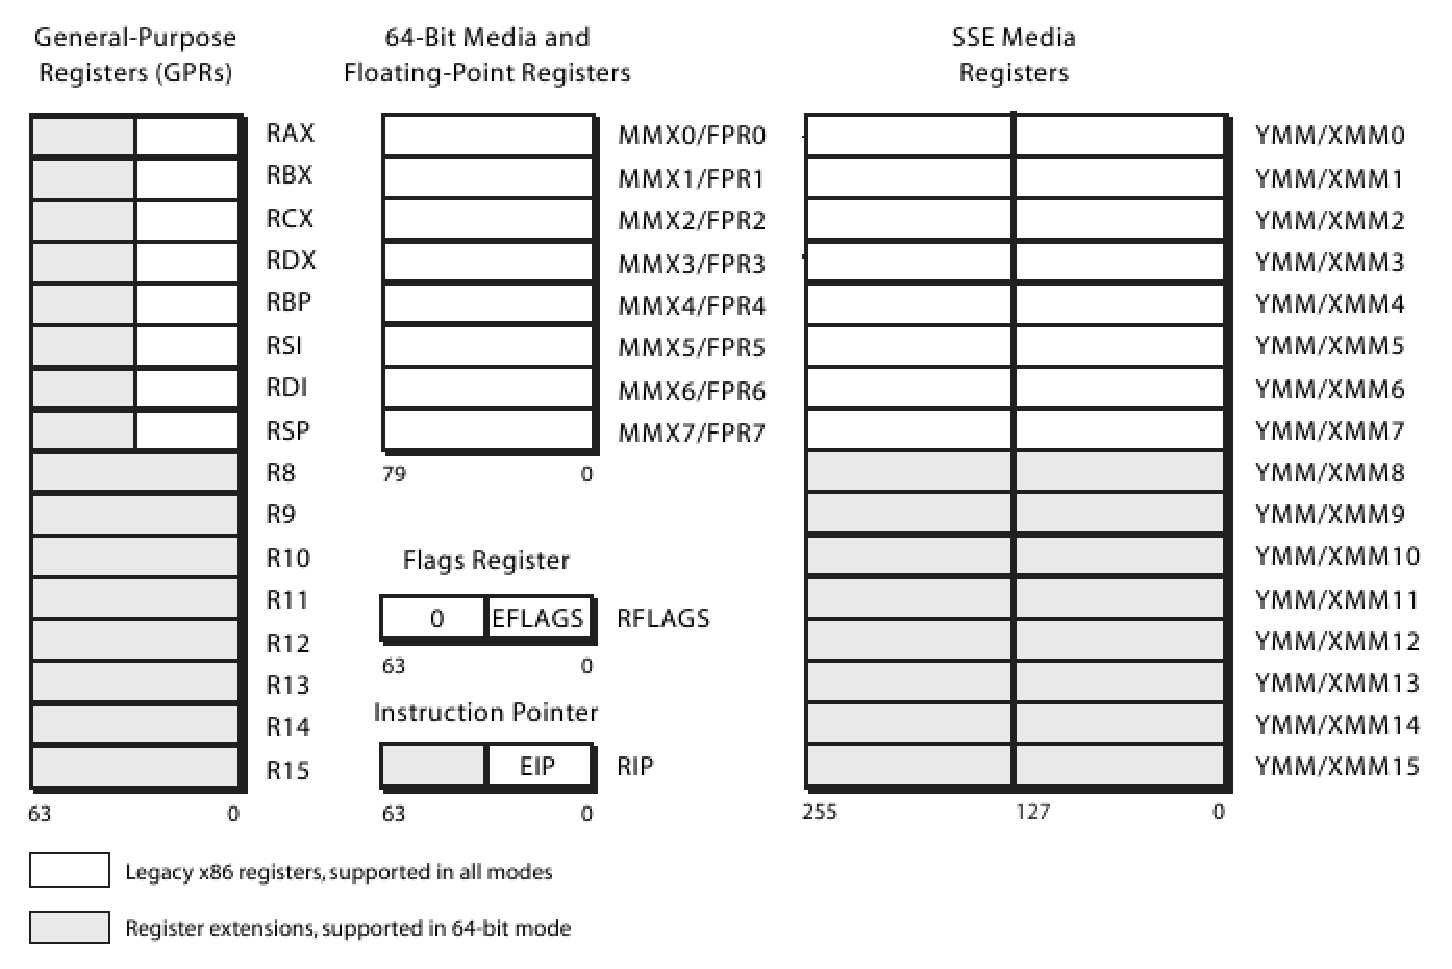
\includegraphics[scale=0.65]{./figures/registers.eps}
\caption{AMD64 Registers}
\label{fig:registers.eps}
\end{figure}


~\figurename{~\ref{fig:registers.eps}} shows the AMD64 application-programming register set. They include the general-purpose registers (GPRs), segment registers, flags register (64-bits), instruction-pointer register (64-bits) and the media registers. 

\subsection{MODES OF OPERATION}
In addition to the x86 legacy mode, another major feature of AMD64 for is its long mode. This is the mode where a 64-bit application (or operating system) can access 64-bit instructions and registers.%~\figurename{~\ref{fig:modes.eps}} shows the features of each mode of operation in AMD64 architecture. 
The different modes of operations in AMD64 architecture are detailed below:
%\begin{tabular}
%\figurename{} 
%\begin{figure}[h!]

%\centering
%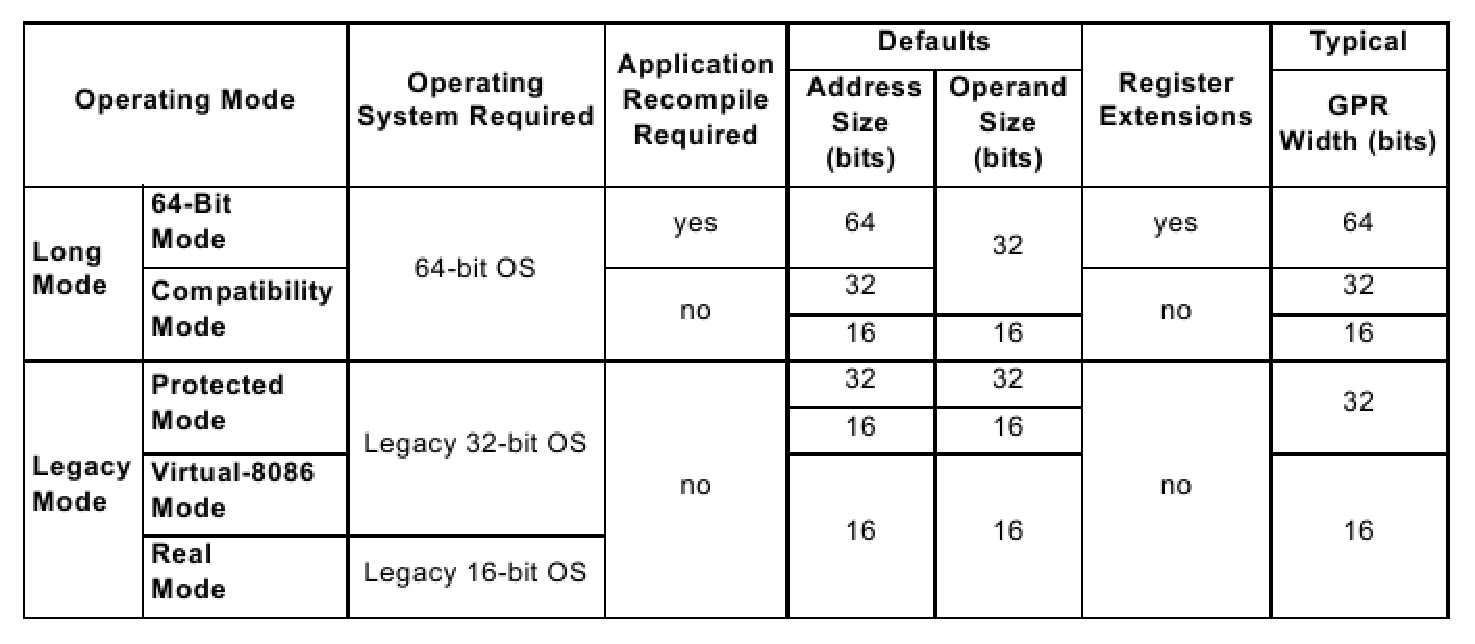
\includegraphics[width=6in]{./figures/modes.eps}
%\caption{AMD64 Modes of Operation}
%\label{fig:modes.eps}
%\end{figure}
%\end{tabular}



\emph {\bf Long Mode}: Long mode is an extension of legacy protected mode. It consists of two sub modes: 64-bit mode and compatibility mode. 64-bit mode supports all of the new features and register extensions of the AMD64 architecture. Compatibility supports binary compatibility with existing 16-bit and 32-bit applications. Long mode does not support legacy real mode or legacy virtual-8086 mode, and it does not support hardware task switching.
\begin{itemize}

\item 64-bit mode: 64-bit mode supports the full range of 64-bit virtual-addressing and register-extension features. This mode is enabled by the operating system on an individual code segment basis. As 64-bit mode supports a 64-bit virtual-address space, it requires a 64-bit operating system and tool chain.


\item Compatibility Mode: Compatibility mode allows 64-bit operating systems to run existing 16-bit and 32-bit x86 applications. These legacy applications run in compatibility mode without recompilation. This mode is also enabled by operating system on an individual code segment bases as in 64 bit mode. However unlike 64-bit mode, x86 segmentation function similar to legacy x86 architecture using 16-bit or 32-bit protected mode semantics.

\end{itemize}



\emph {\bf Legacy Mode}: Legacy mode has compatibility existing 16-bit and 32-bit operating systems in addition to compatibility with existing 16-bit and 32-bit application. Legacy mode has the following three submodes : 

\begin{itemize}

\item Protected Mode: Legacy protected mode supports 16-bit and 32-bit programs with memory segmentation, optional paging, and privilege-checking. Programs in this mode can access up to 4GB of memory space.


\item Virtual-8086 Mode: Virtual-8086 mode supports 16-bit real-mode programs running as tasks under protected mode. It uses a simple form of memory segmentation, optional paging and limited protection-checking. Programs in virtual-8086 mode can access up to 1MB of memory space.


\item Real Mode: Real mode supports 16-bit programs using register-based memory segmentation. It does not support paging or protection-checking. Programs running in real mode can access up to 1MB of memory space.
\end{itemize}

\section{MEMORY ORGANIZATION}
\addtocontents{toc}{\protect\setcounter{tocdepth}{1}}

The AMD64 architecture organizes memory into virtual memory and physical memory~\citep{SS:AMD64-V2}. Virtual memory and physical-memory spaces are usually different in size with virtual address space being much larger than physical-address memory.  System software relocates applications and data between physical memory and the system hard disk to make it appear that much more memory is available than what really exist and then uses the hardware memory-management mechanisms to map the larger virtual-address space into the smaller physical-address space.

\subsection {VIRTUAL MEMORY}
Virtual memory consists of the entire address space available. It is a large linear address space that is translated to a smaller physical address space. Programs uses virtual address space to access locations within the virtual memory space. System software is responsible for managing the relocation of applications and data in virtual memory space using segment-memory management. System software is also responsible for mapping virtual memory to physical memory through the use of page translation.

The architecture supports different virtual-memory sizes using the following modes:
\begin{itemize}

\item[-] Protected Mode: Supports 4 gigabytes of virtual-address space using 32-bit virtual  addresses.

\item[-] Long Mode: Supports 16 exabytes of virtual-address space using 64-bit virtual addresses.
\end{itemize}

\subsection {PHYSICAL MEMORY}
Physical addresses are used to directly access main memory. This is the installed memory in a particular system that can be physically accessed by the bus interfaces. The larger virtual address space is translated to smaller physical address space through two translation stages called segmentation and paging. The architecture supports different physical-memory sizes using the following modes:
\begin{itemize}

\item[-] Real Mode- Supports 1 Megabyte of physical-address space using 20-bit physical addresses.
\item[-] Legacy Protected Mode- Supports several different address-space sizes, depending on the translation. supports 4 gigabytes of physical address space using 32-bit physical addresses and when the physical-address size extensions are enabled, the page-translation mechanism can be extended to support 52-bit physical addresses.
\item[-] Long Mode- Supports up to 4 petabytes of physical-address space using 52-bit physical addresses. Long mode requires the use of page-translation and the physical-address size extensions (PAE).
\end{itemize}

\section{MEMORY MANAGEMENT}

\addtocontents{toc}{\protect\setcounter{tocdepth}{1}}

Memory management refers to the process involved in translating address generated by software to physical address through segmentation and paging. This process is hidden from application software and is handled by system software and processor hardware. 

\subsection{SEGMENTATION} 
Segmentation mainly helps system software to isolate software processes (tasks) and the data used by that process to increase the reliability of system running multiple process simultaneously. The AMD64 architecture is designed to support all forms of legacy segmentation. In 64-bit mode segmentation is not adopted (use flat band segmentation). Segmentation is, however, used in compatibility mode and legacy mode. 
~\figurename {~\ref{fig:segmentation.eps}} shows segmented virtual memory.

%\figurename{} 
\begin{figure}[H]
\centering
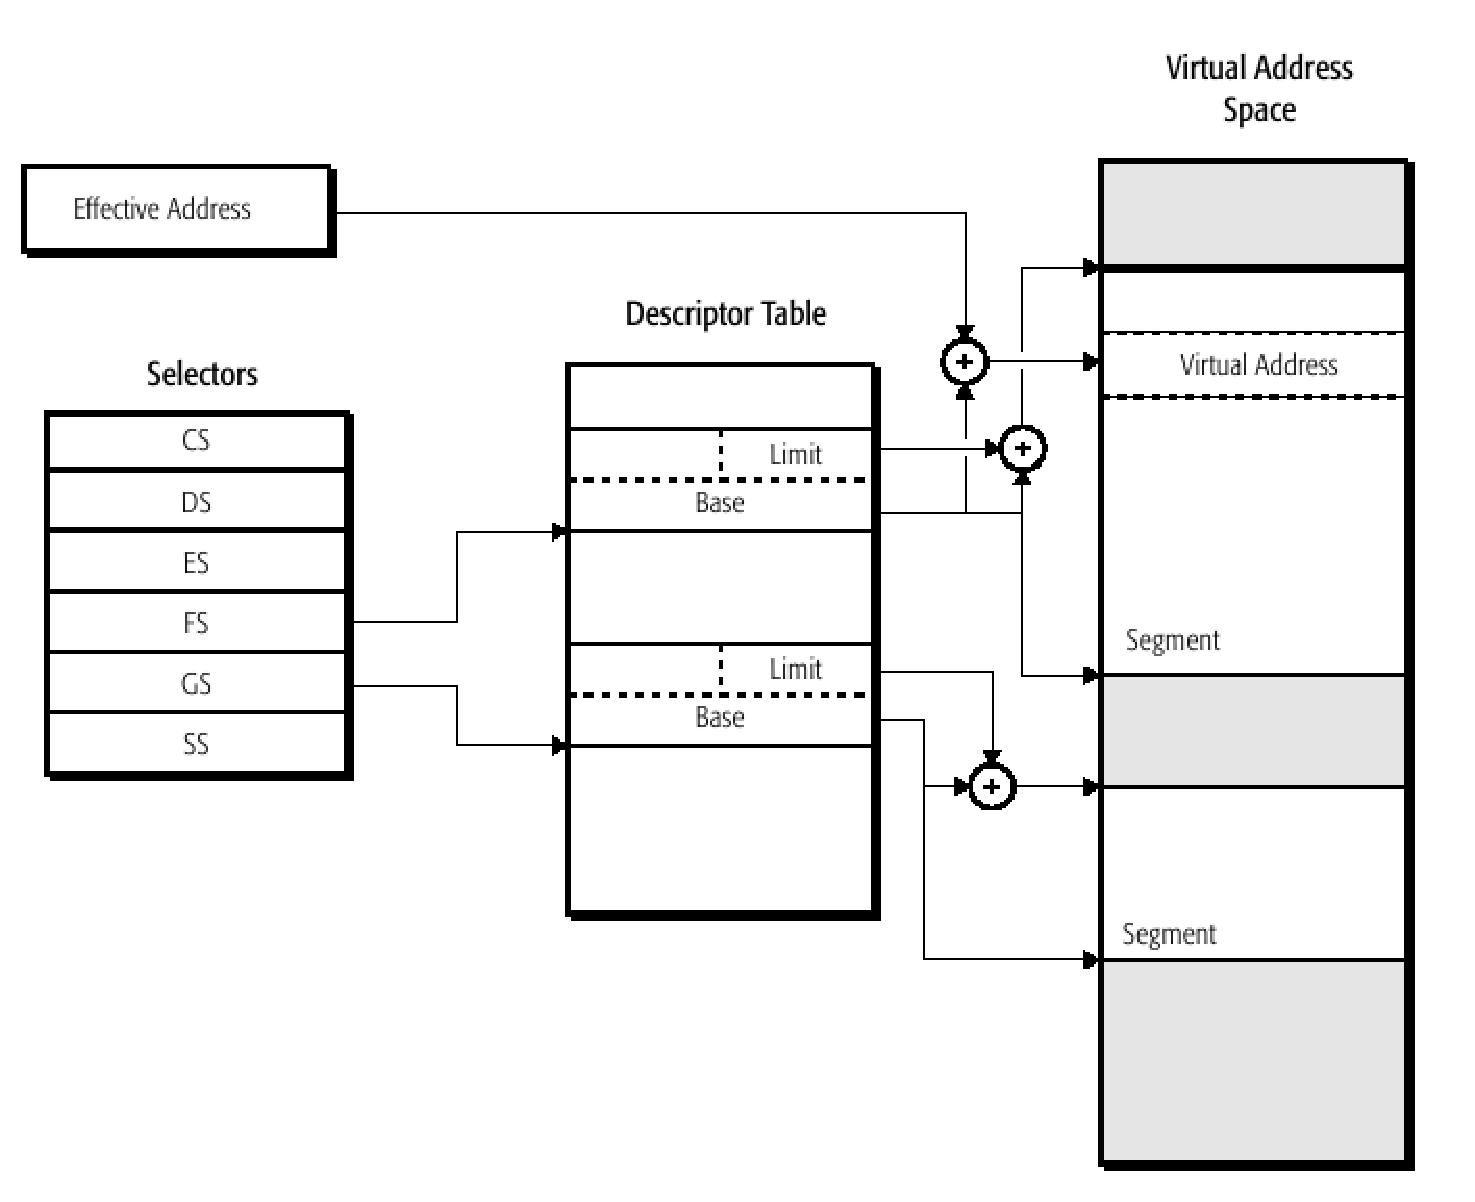
\includegraphics[scale=0.5]{./figures/segmentation.eps}
\caption{Segmented Memory Model}
\label{fig:segmentation.eps}
\end{figure}


The segmentation mechanism provides ten segment registers, each of which defines a single segment. Six of these registers (CS, DS, ES, FS, GS, and SS) define user segments. The remaining four segment registers (GDT, LDT, IDT, and TR) define system segments. The segment selector points toward a specific entry in descriptor table. This can be Global Descriptor Table (GDT) or Local Descriptor Table (LDT). The descriptor table entry base value plus the effective address which is the offset from base gives the virtual address. Effective address is calculated from the value stored in general purpose register and a displacement value encoded as part of instruction.

\subsection{PAGING}
Paging allows software and data to be relocated in physical address space using fixed-size blocks called physical pages. It translation uses a hierarchical data structure called a page-translation table to translate virtual pages into physical pages. Paging also provides protection as access to physical pages by lesser-privileged software can be restricted. ~\figurename {~\ref{fig:paging.eps}} shows an example of paged memory with three levels in the translation-table hierarchy. 




%\figurename{} 
\begin{figure}[H]
\centering
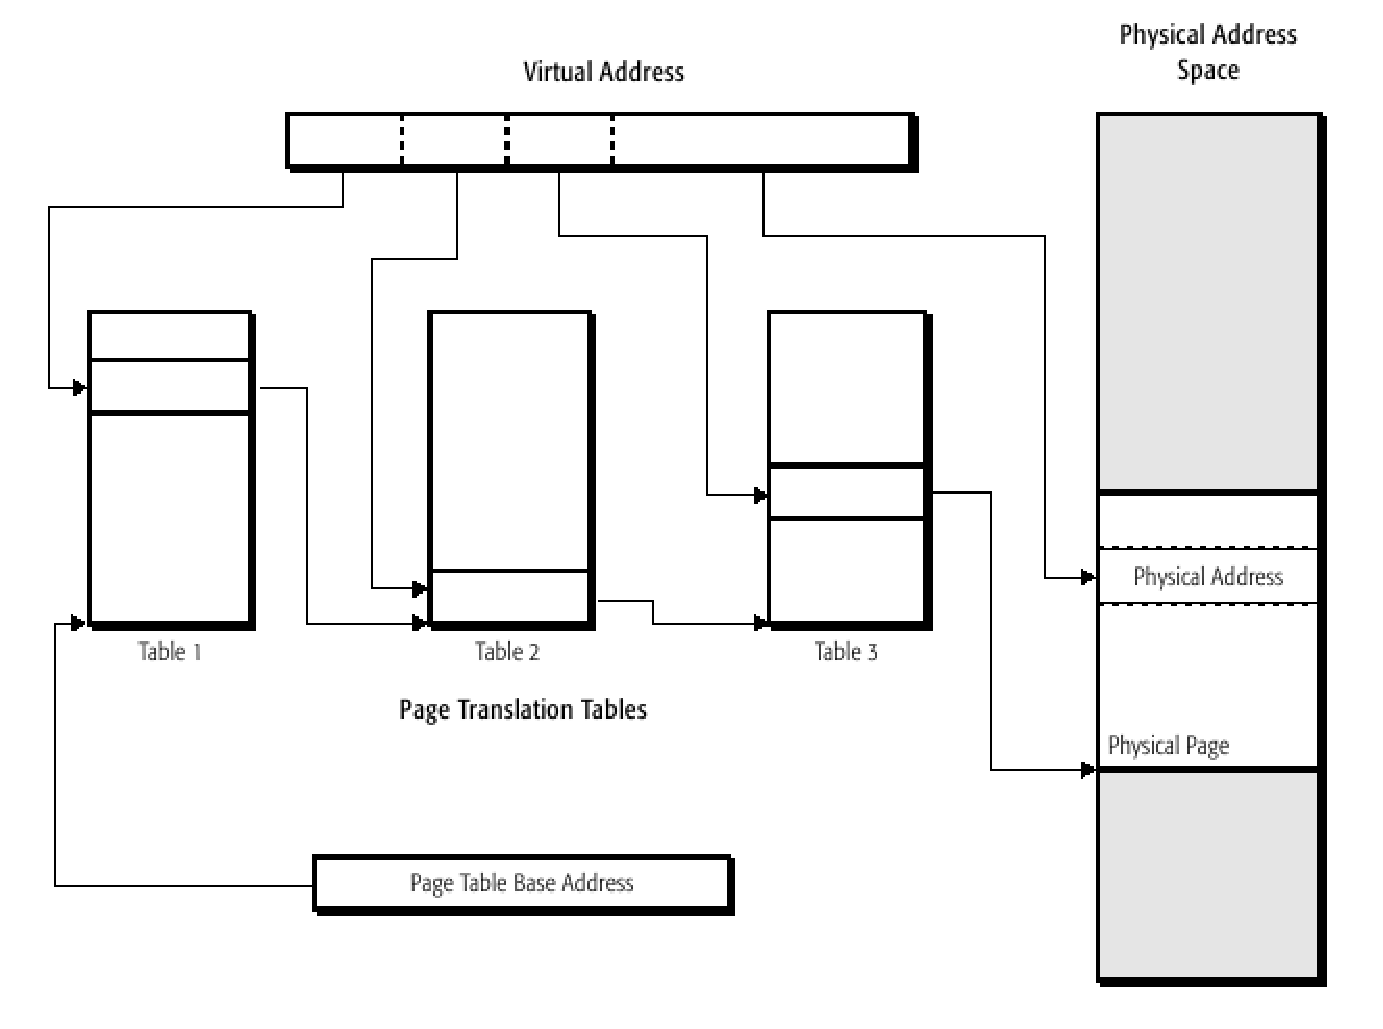
\includegraphics[scale=0.5]{./figures/paging.eps}
\caption{Paged Memory Model}
\label{fig:paging.eps}
\end{figure}



The number of levels in the translation-table hierarchy can be as few as one or as many as four, depending on the physical-page size and processor operating mode. Each table in the translation hierarchy is indexed by a portion of the virtual-address bits. The entry referenced by the table index contains a pointer to the base address of the next-lower level table in the translation hierarchy. Last page table entry plus the offset value from the virtual address (lsb bits), points toward the actual physical address.  


%%%%%%%%%%%%%%%%%%%%%%%%%%%%%%%%%%%%%% VERIFICATION ENVIRONMENT %%%%%%%%%%%%%%%%%%%%%%%%%%%%%%%%%%%%%%%%%%%%%%%
\newpage
\chapter{VERIFICATION ENVIRONMENT}
\label{chap:verification.tex}

\section {FUNCTIONAL VERIFICATION}

In SoC design methodology, the first step is to define the specifications. Once enough system specification is available, design phase starts. The behavioral modeling of the design is done using hardware description languages like VHDL or Verilog HDL and in this stage the design is said to be Register Transfer Level (RTL)\nomenclature{RTL}{Register Transfer Level}. Such design could be partitioned to aid reusability, concurrent development and tool effectiveness. In general, reusable components of designs are packaged into components called Intellectual Property (IP). The RTL description of design is verified against functional specifications. System level verifications are done to verify the RTL description against the intended functionality among other requirements such as timing, power and gate-count. 



Functional verification validates that the design meets its requirements. Test cases are created based on specifications. Various aspects of data and control flow are verified by passing information between external environments, communication with I/O devices,  software interactions etc. 
 
\section {VERIFICATION}

Most SoC verification concentrates on verifying the processor cores and their interactions with SoC level IPs. At this level of abstraction, verification is concentrated on interaction between IPs and on design features those haven't got verified as a sub-system.  Test conditions are written in x86 assembly or in some cases written in high level languages like {\it C++}. The intention of each test is to verify specific functionality of the design and ensure its validity. Test plans must be in sync with specifications and are required to be updated when specifications change. Test methodology should also be adaptable to accomodate such changes and to deal with all possible corner cases and boundary conditions.

Tests are developed, so that they stimulate the design in a specific manner and compare outcome against expected outcome to assert accuracy of design behaviour. Ideally design should be verified against all possible scenarios that could arise and once it passes all tests, it can be considered as completely verified. In case when a particular test fails, the verification engineer needs to find out the cause of failure with his understanding of design or verification aspect that led to the particular failure. This process of root causing a failure is called as a ``{\it debug}'' in verification. Once root-caused, the engineer then has to suggest appropriate changes to either design, verification or documentation to keep them in unison. 

There are many possible issues that can lead to a test failure. Each test defines conditions for pass and fail. A fail or pass is basically the outcome of a test run. There can be different causes for failures, with majority of them being:

\begin{description}
	\item[Self check fails:] In a self check failure, the program code running on the simulated processor is able to identify and report a failure. The program tests are written such that they evaluate the results, compare it with desired value and finally report fail or pass. 
	\item[Assertion/Checker fails:] Assertion or checker fails are very common kind of failures and occur when a test-bench component reports an unexpected behaviour of the design. It could also be a false failure. In general, most checkers or assertions monitor particular design states during simulation and report failure whenever monitored value deviates from the expected value. 
\end{description}

In general, a self check fail is caused when program execution deviates from the intended execution flow. Hence the debug of a self check fail would require knowledge of the program under test and its intended execution flow. Without this knowledge, it would be a challenge to debug such fails. This project is aimed to improve debug of such self check fails.

%\subsection {DEVELOP TESTS}
%
%Tests for verifying all the features of the RTL are written in x86 assembly or in high level languages. These test plans are in sync with the specifications of RTL and are to be updated with new specification changes. Test cases should be efficient enough to deal with all possible []: 
%\begin{itemize}
%
%\item Corner cases
%\item Boundary conditions
%\item Design discontinuities
%\item Error conditions
%\item Exception/Interrupt handling
%
%\end {itemize}

\subsection {SELF CHECK FAILURE}

Processor tests are C/assembly program written to assert that the processor under test is indeed functioning as expected under that specific setup. These processor tests are designed such a way that they are capable of deciding if the processor execution results were successful. These tests are normally hand written by the verification engineer rather than randomly generated.  Hence such tests can string together specific stimulus of interest and determine pass or fail status on its own without relying on other verification components. Such tests are called as ``self-tests''.


%\figurename{} 
\begin{figure}[h]
\centering
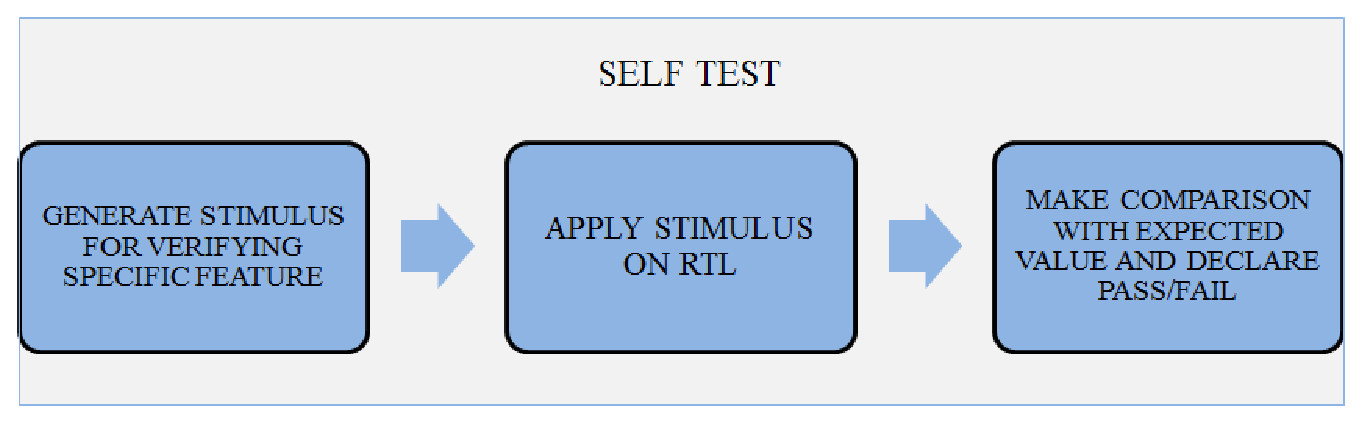
\includegraphics[scale=0.65]{./figures/selftest.ps}
\caption{Self-Test} 
\label{fig:selftest.ps}
\end{figure}

\figurename~{\ref{fig:selftest.ps}} details the flow of a self-test. Self-tests are a collection of x86 assembly language program. Tests are compiled by a script which calls an assembler followed by a linker. The final output being a linked binary image that can be loaded and executed by the RTL model of DUT\nomenclature{DUT}{Design Under Test}. Stimulus is generated by the test and is applied to the DUT. Comparisons are done by the test itself after which pass/fail result is generated.



\section{DEBUGGING A SELF CHECK FAILURE}

Self-tests report the occurrence of test case failure. Once this is available, next step is to analyze the reason for failure.  For this, a traceback from the point of failure to the point of error is required. 

A failure message would indicate which check failed that the result is deviating from the desired value. This desired value can be understood from analysing the asm test code. But to understand at which point during execution the design deviated from desired course, detailed information regarding execution flow as well as a reference flow which has the ideal values and status are required. In general, a reference flow could be established by the engineer after understanding and interpreting the test in its completeness.
 
To aid execution flow, RTL is simulated along with an instruction level reference emulator. The reference emulator is a software model which imitates the design functionally and executes same instructions in parallel with the RTL. This parallel simulation is also called as model cosimulation and produces a log of processor activity.


\subsection {MODEL COSIMULATION}
The instruction level reference emulator (ILE) \nomenclature{ILE}{Instruction Level Emulator} is an x86/x86-64 compatible model, generally written in software languages such as {\it C++}. It models the processor in great detail including registers, caches and modes of operation. The test provides stimulus to both the RTL and reference models. An interface between RTL and reference model compares the states after each instruction retire and reports any mismatches, if any. 

Following sections describes features and functions of emulator and interface. 



%\figurename{} 
\begin{figure}[h]
\centering
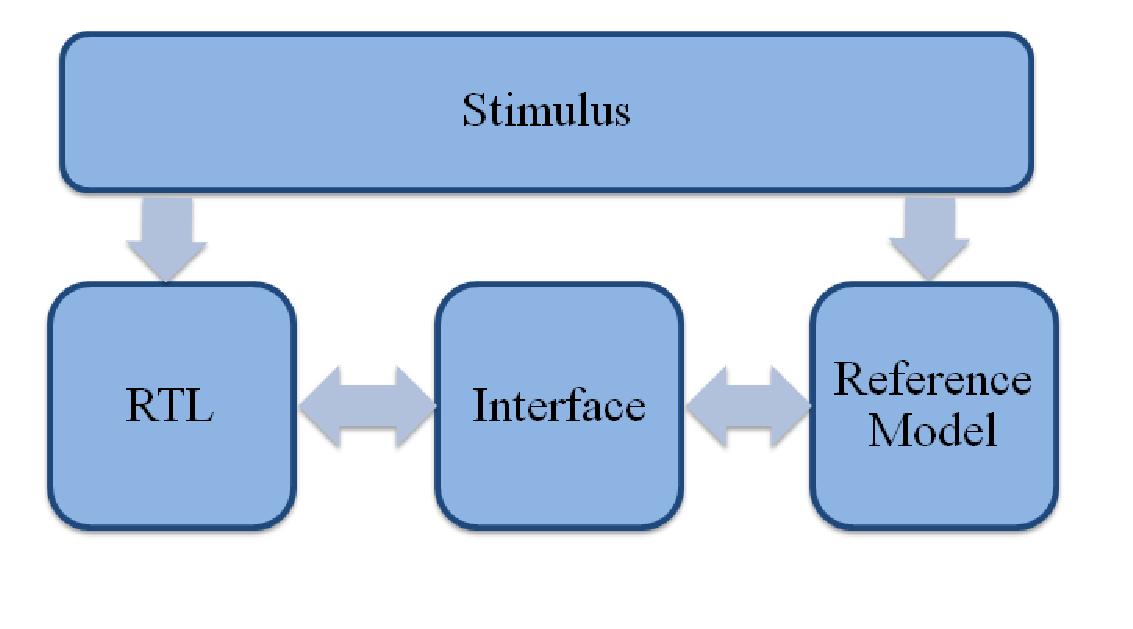
\includegraphics[scale=0.65]{./figures/interface.ps}
\caption{RTL-Reference Model Cosimulation} 
\label{fig:interface.ps}
\end{figure}



%\subsection {COMPARISON WITH REFERENCE MODULE}

%The RTL is simulated along with an instruction level reference emulator. This instruction level emulator is an x86/x86-64 programming model. It mainly models the register states and memory features and act as the ideal reference point to compare with. An interface between RTL and reference model compares the states after each instruction retire and report any mismatch. The following section details the features and functions of emulator and interface.

\subsubsection {INSTRUCTION LEVEL EMULATOR}
The x86 ILE starts emulation after initializing the contents of its memory with linked binary image of the test. The ILE emulates the fetch/decode/execute algorithm of a scalar processor, producing an output log known as {\it processor execution log}. Each log entry describes the instruction, its results and any side effects it had on the processor state. The emulator models debug features, exceptions and interrupts as well as processor specific features. Supported processor states include x86 general purpose registers, flag registers, control registers, media registers, model specific registers as well as memory and I/O spaces. The emulator runs multithreaded code to simulate multiprocessor and multicore processor systems.\\ 
The emulator runs in step with the RTL. Whenever an instruction or exception is retired in RTL that thread within the emulator is stepped-up and the processor states in the RTL and the emulator are compared. Difference detected in processor states are considered as a {\it mismatch}; difference in memory locations are also considered as {\it memory mismatches} and upon any {\it mismatch}, the cosimulation is terminated. At the end of RTL simulation when all threads stop executing, the memory states of RTL and the emulator are compared and any discrepancies are reported as memory mismatches.

\subsubsection {INTERFACE}
The interface connects RTL and reference model, and helps to keep the ILE in step with RTL signal. It steps the ILE when an instruction in RTL simulation has retired and then compares the results of execution between RTL and ILE. If the reference model is unable to model anything that is present in the RTL, the interface also re-synchronizes the ILE with the state obtained after execution of the RTL instruction.
Main functions of this interface includes:
\begin{description}
	\item[Initialization:] Initialize memory model, attach with RTL and ILE, and initialize some specific RTL signals.
	\item[Increment:] Based on number of instruction retired per cycle, the interface informs ILE how many instructions to step.
	\item[Interrupt Handling:] Interface informs ILE about pending interrupts.
	\item[Comparing:] Compares RTL and reference model registers; integer, FP, control and status word. Also reports any mismatches.
	\item[Interfacing with the memory model:] Tell memory model what operations are seen by the RTL. 
\end{description}

\label{verif:exelog}

During the course of emulation, the ILE generates log files containing processor's program execution details. These are called {\it processor execution logs}. These log files contains cycle by cycle information regarding register states, memory values, flags, threads etc. These log entries help debug in the event of failure.
%The  generated by ILE, during the course of emulation, contains cycle by cycle information regarding register states, memory values, flags, threads etc. All the comparisons and debugging requires these information.

On the event of a failure, emulation terminates and and debugging is required. In order to root-cause the failure, verification engineer needs to trace through this {\it processor execution log}. Mismatches with reference model values provide information regarding the cause of failure.

Tracing through the log files is done manually. Data obtained from {\it processor execution log} and the assembled test files needs to be analyzed and correlated for debugging the failure. This is a very tedious effort consuming a lot of verification time. This is because of two main reasons:

\begin{enumerate}
	\item Relevant/required information is buried under a wealth of information.
	\item Correlated information is spread across in different files.
\end{enumerate}

As the design itself is very complex, these reasons makes manual tracing too time consuming. This stretches the verification time and ultimately time-to-market.   


 

%%%%%%%%%%%%%%%%%%%%%%%%%%%%%%%%%%%%%% PROPOSED ENHANCMENT %%%%%%%%%%%%%%%%%%%%%%%%%%%%%%%%%%%%%%%%%%%%%%%
\newpage
\chapter{PROPOSED ENHANCEMENT}
\label{chap:enhancement.tex}

\section {PROCESSOR EXECUTION DETAILS}

During simulation of a processor core, the linked program image is loaded in processor's memory followed by its execution. Most modern microprocessors adopt instruction level parallelism for high throughput. Micro-architectural features like instruction pipeline, superscalar execution, register renaming, speculative execution, branch prediction etc. are employed in order to exploit instruction level parallelism.  These micro architecture features work together for high execution throughput. All these internal operations results in a complex execution flow with multiple operations happening in each cycle with different levels of dependencies between data, instruction and memory.


As explanined in Section~\ref{verif:exelog} execution log file captures important information regarding the processor state and activity during execution of program code. This could be considered as history of events in the simulation. Each entry in the log file contains the following information regarding processor execution:
\begin{itemize}
	\item The instruction number, simulation cycle and opcode
	\item Thread Id (relevant in multi-core and multi-processor)
	\item Memory read/write information
	\item Code read/write
	\item I/O read or write
	\item Interrupt and exception information
	\item Branch Target
	\item Paging info
	\item Flag values
	\item Register affected on that instruction execution
\end{itemize}
On the onset of simulation failure, these information are vital in debugging the cause of a failure. The following case study of two test scenarios affirm this fact.

\section {SAMPLE DEBUG CASES IN CONSIDERATION}
\label{sec:enhancement.tex.sdcic}
Let us consider two simple assembly tests as case studies to demonstrate the usefullness of processor execution log during debug of a self~test failure.
\subsection {TEST A}
\label{case:testa}

%\vspace{1.5cm}


\IncMargin{1em}
\begin{algorithm}[h]
\DontPrintSemicolon
\SetKwInOut{Input}{Input}\SetKwInOut{Output}{Output}

\Input{$data$, $address$}
\Output{Test result: $pass$ or $fail$}
\BlankLine
Initialization: Select memory bank by setting $Control Register$ \;

	$Reg A \longleftarrow data$\;
	$Reg B \longleftarrow address$\; \label{algo:mrw:write}

	Memory $[Reg B] \longleftarrow Reg A $\;

	$Reg D \longleftarrow$	Memory $[Reg B]$\;  \label{algo:mrw:read}

\eIf{$Reg A == Reg D$}{ \label{algo:mrw:compare}
report $pass$
}{
report $fail$
}

\caption{Memory Read-Write}
\label{algo:mrw}
\end{algorithm}\DecMargin{1em}

%\vspace{1.5cm}

Consider an assembly test in Algorithm~\ref{algo:mrw} that intends verification of a memory module. The test writes a value into a memory location (Line~\ref{algo:mrw:write}). The data is later read from the same location (Line~\ref{algo:mrw:read}) and compared with the original value written into the location (Line~\ref{algo:mrw:compare}). The test flags fail or pass based on the comparison.

The test verifies a single write/read from a memory location. Ideally the values written to the memory location should match the value read from the memory and test completes with a pass. Now consider a case where the comparison fails. This could occur due to many reasons. Following are a few scenarios which can lead to a failure:
\begin{itemize}
\item [Case 1]: If from another thread of program execution, the control bit for bank selection is changed during the execution, the data read will be from wrong memory location, leading to a failure. \label{algo:mrw:case1}

\item [Case 2]: If the address value is invalid. This can happen when the test generates a random address value for storing the data and this value might not exist in the current selected memory bank range. \label{algo:mrw:case2}

\item [Case 3]:  If the register $Reg D$ chosen is unavailable in this mode of processor operation. This will cause the wrong data to be updated into the memory and comparison fails. \label{algo:mrw:case3}
\end{itemize}

\subsubsection{Debug Process}
In case~1~\ref{algo:mrw:case1}, the memory bank selected should stay same throughout the program execution. Any change in memory bank selects will cause the read operation to take value from wrong memory block, leading to a self-test failure.
In case~2~\ref{algo:mrw:case2}, given that each memory block has a fixed size, if the generated random address generated is not in valid range of offset, then this error could occur.
In case~3~\ref{algo:mrw:case3}, if care is not taken in choosing processor mode prior to the test execution, and if $Reg D$ is either completely or partly unavailable (like 32~bit mode Vs 16~bit mode), then this error could occur.

\begin{figure}[h]
\centering
\includegraphics{./figures/mrw_debug.ps}
\caption{Illustration of debug process : Test A} 
\label{fig:mrw_debug.ps}
\end{figure}

\figurename{\ref{fig:mrw_debug.ps}} depicts a typical debug process. Note that there could be other causes for failure as depicted in $states \textcircled{j}, \textcircled{k}, \& \textcircled{m}$. During debug, the engineer needs access to certain information as listed here
\begin{enumerate}
\item $state~\textcircled{b}$: Examine Read to address, examine data obtained.
\item $state~\textcircled{c}$: Obtain all accesses occurred to same address, find the latest write to same address.
\item $state~\textcircled{d}$: Examine data written to latest write to same address.
\item $state~\textcircled{e}$: What is the bank select location, did it change between write and read.
\item $state~\textcircled{f}$: Which program code changed bank select?
\item $state~\textcircled{l}$: What is processor mode?
\item $state~\textcircled{i}$: What was the random address that got generated?
\end{enumerate}

\subsection {TEST B}
\label{case:testb}
Consider a string $tolower()$ program. The program reads an input string in upper~case and converts it to lower~case. Considering ASCII character encoding, conversion of upper~case to lower~case could be accomplished by addition of constant to the ASCII encoding.



%\vspace{1.5cm}
\IncMargin{1em}
\begin{algorithm}[h]
\DontPrintSemicolon
\SetKwInOut{Input}{Input}\SetKwInOut{Output}{Output}

\Input{$string$}
\Output{$string$}
\BlankLine
 \For{every character $c$ in string}{\;
  $c \longleftarrow c + CONST $\;
 }\;

\caption{String Lower Case Conversion}
\label{algo:lcc}
\end{algorithm}\DecMargin{1em}

%\vspace{1.5cm}

The program in Algorithm~\ref{algo:lcc} converts each character from upper case to lower case in a loop, to achieve the result. This program can fail due to many reasons. Let us consider a couple of scenarios.

\begin{itemize}

\item [Case 1]: Consider that the loop variable is not initialised incorrectly. Loop variables are used as the index variable to select every character of the string. This will lead to an invalid conversion. \label{algo:tolow:case1}

\item [Case 2]: If loop exit condition is wrong, then the loop could terminate early. \label{algo:tolow:case2}
\end{itemize}

\subsubsection{Debug Process}

In case~1~\ref{algo:tolow:case1}, initialisation of loop variable is the cause and could be found by looking at value of the variable just after loop is entered. If after the completion of loop execution for the first time, if the first character remains un-modified, then that also suggests an initialisation problem.
In case~2~\ref{algo:tolow:case2}, the resulting string after loop exit would normally have characters unmodified towards the end. This case could be identified with such symptom.

\begin{figure}[h]
\centering
\includegraphics{./figures/tolower_debug.ps}
\caption{Illustration of debug process : Test B} 
\label{fig:tolower_debug.ps}
\end{figure}

\figurename{\ref{fig:tolower_debug.ps}} depicts a typical debug process for this case. Note that there could be other causes for failure as depicted in $state~\textcircled{g}$. During debug, the engineer needs access to certain information as listed here

\begin{enumerate}
\item $state~\textcircled{b}$: Find address of loop var.
\item $state~\textcircled{c}$: At start of loop, check initial value of loop var.
\item $state~\textcircled{d}$: When the loop exited, what was the value of loop var.
\item $state~\textcircled{e}$: Need computation values of loop exit condition.
\item $state~\textcircled{f}$: Need computation values of loop init condition.
\end{enumerate}

\section {NECESSITY TO ENHANCE MANUAL VERIFICATION}
\label{sec:enhancement.tex.nemv}

Debug engineer has to extract required information whenever needed, manually from assembly files, linked object files and processor execution logs. Correlation of information between different files is also required to make a successful debug. Such manual extraction of information and correlation of it, though may seam obvious consumes considerable debug time and is error prone. Hence an enhancement to such manual process, if available, would considerably decrease the time required to debug an issue.

Information exists in processor execution log, assembly file and list file. Correlation of list file and execution log file can be accomplished by correlating address. For each cycle the Instruction pointer register (RIP) hold the current and next instruction address. The verification engineer has to search through the files for address values to correlate cycles in log file with lines in list file. As observed in Section~\ref{sec:enhancement.tex.sdcic}, data extraction and correlation from different files are required at different stages of debug to effectively debug how and why the test failed.

\section {ENHANCING MANUAL VERIFICATION}
\label{sec:enhancement.tex.emv}

After analysing debug process, it is very evident that availabitily of correlated information while during debug process would enhance it in a big way.  In this thesis, we are proposing a Graphical User Interface (GUI) which will help in navigating through the log files quickly, aiding in comparison with list file and also some additional features to help in faster analysis of failure cause. The interface will help to get rid of traditional method of comparing Instruction Pointer Register (RIP) values and string search by providing graphs that will connect each cycle in log file with corresponding asm line code. The proposed interface enhances the data navigation through log files and failure analysis.  It is possible to lay down the requirements of such an enhancement

\begin{description}
\item[Visualisation of Execution Flow] Visual representation of data is always very appealing, than without a visual representations. In our case, if there exists a visual representation of execution control flow, it would be obvious if a loop had executed and if so, how many times it was.
\item[Navigating Execution Flow] In the visual representation of execution flow, it would also aid deubg when user is able to navigate to point of interest by mouse~guestures on such representation. For eg. if program code exists across different source files, the user would be able to navigate to the point of interest with ease.
\item[Processor State Information] At any exeuction point, it would help the debug engineer if processor state information such as SP\nomenclature{SP}{Stack Pointer}, PC\nomenclature{PC}{Program Counter}, SR\nomenclature{SR}{Status Register} are readily accessable.
\item[Processor State Information Change] It would aid debug to be able to list the differences in Processor State Information between two arbitary points of execution.
\item[Processor Writes and Reads] It would aid debug if processor writes and reads could be easily listed. It would also help if in such listing one could classify between IO accesses and memory accesses.
\item[Code listing] It would aid debug when source code is listed along with its context, on any point of execution.
\end{description}

%In general for different test and error possibilities, all information regarding the processors execution flow is required. From the point of failure, a trace back through the execution log details and corresponding comparison with the expected assembly code action must be made. 
%The above cases show that main aspect of failure analysis is co-relating the execution information with the test code and tracing the execution flow. 
%
%\section{Co-relating information}
%
%
%\section{Tracing the log files}
% 
%As explained earlier, processor execution logs are generated during test simulation. These files hold almost all details that can be possibly identified during simulation. 
%
%In SoC level verification, each simulation will have a collection of many tests verifying intimate details of the design. The test plans will have many small tests and will be a big collection and have thousands of code lines. 
%In such cases it is rather obvious that the execution log file for such tests stimulus will be huge as it covers cycle by cycle processor details.  This vast wealth of information will be in generated in a simulation time based manner with details of various threads mixed together. 
%
%During debug the verification engineer need to trace the log file contents to find out the cause of failure. This navigation through such huge file can be a very tedious process if done manually by calculating linear address and then using string search to find the address in log file and asm file to correlate.  In fact the data traversal can move up and down for verifying different aspects. This will consume a lot of verification time. 
%


 

%%%%%%%%%%%%%%%%%%%%%%%%%%%%%%%%%%%%%% INTERFACE IMPLEMENTATION %%%%%%%%%%%%%%%%%%%%%%%%%%%%%%%%%%%%%%%%%%%%%%%
\newpage
\chapter{INTERFACE IMPLEMENTATION}
\label{chap:GUI_impl.tex}
\section{INTERFACE}
The necessity to enhance manual debug methodology has been established in Section~\ref{sec:enhancement.tex.nemv} and certain requirements of such an interface is established in Section~\ref{sec:enhancement.tex.emv}. This chapter concentrates on design and implementation of the debug interface.

The debug interface is aimed at being intuitive and user friendly. It should aid data navigation so as to reduce manual efforts. If user requires to refer to actual processor execution log or assembly code, it should be readily available through the interface. The interface should also provide graphical representation of processor execution log, to aid traversal and filtering of processor activity. The interface should aid traversing through processor execution easy.  Critical events made by processor should be extracted, categorized and made available to user.

In addition to interface requirements listed in Section~\ref{sec:enhancement.tex.emv}, the following set of features would also aid in debug:

\begin{itemize}
\item[-] Visualizing thread-wise execution flow
\item[-] Ability to highlight instances of critical activities such as Memory write/read, I/O write/read, Branching etc
\item[-] Interrupt and exception happening during execution
\item[-] Assembly code traversal and its linkage with execution flow
\item[-] Register current state value traversal and its linkage with execution flow
\item[-] Comparison of register values between arbitrary instances of execution
\item[-] Simulation cycle of execution event
\end{itemize}

Every stimulus is a unique assembly test and hence the debug interface should be as generic as possible. It should be able to accommodate any relevant assembly test, accompanied with execution logs.

%Once the simulation is completed and failure is reported the debug phase starts. This is where the role of GUI comes. From the vast information provided by the logs and test files, interfaces have to capture and represent relevant information to the user. The following section details the implementation and features of the proposed GUI. 

\subsection {CHOOSING GUI}
There are multitude of languages providing GUI capability, the project dies not need a very sophisticated GUI implementation. Moreover the interface should aid remote debug and if possible thee should not be any requirement for any user to install a tool-kit or library for the debug interface to be used. Hence the decision to use web-browser as the debug interface was a default choice. A web browser could also execute {\it javascripts} and that makes it customisable. The design is also scalable and aids introduction of new features for debug with ease.

Each stimulus will have its own set of assembly test files and execution log files. The interfaces implementation starts by consuming these files. Two programming languages are used for implementation:
\begin{description}
\item[Python Script] for data extraction and correlating related information.
\item[JavaScript] for designing the interface features and user interaction.
\end{description}

\addtocontents{toc}{\protect\setcounter{tocdepth}{2}}
%\figurename{} 
\begin{figure}[h]
\centering
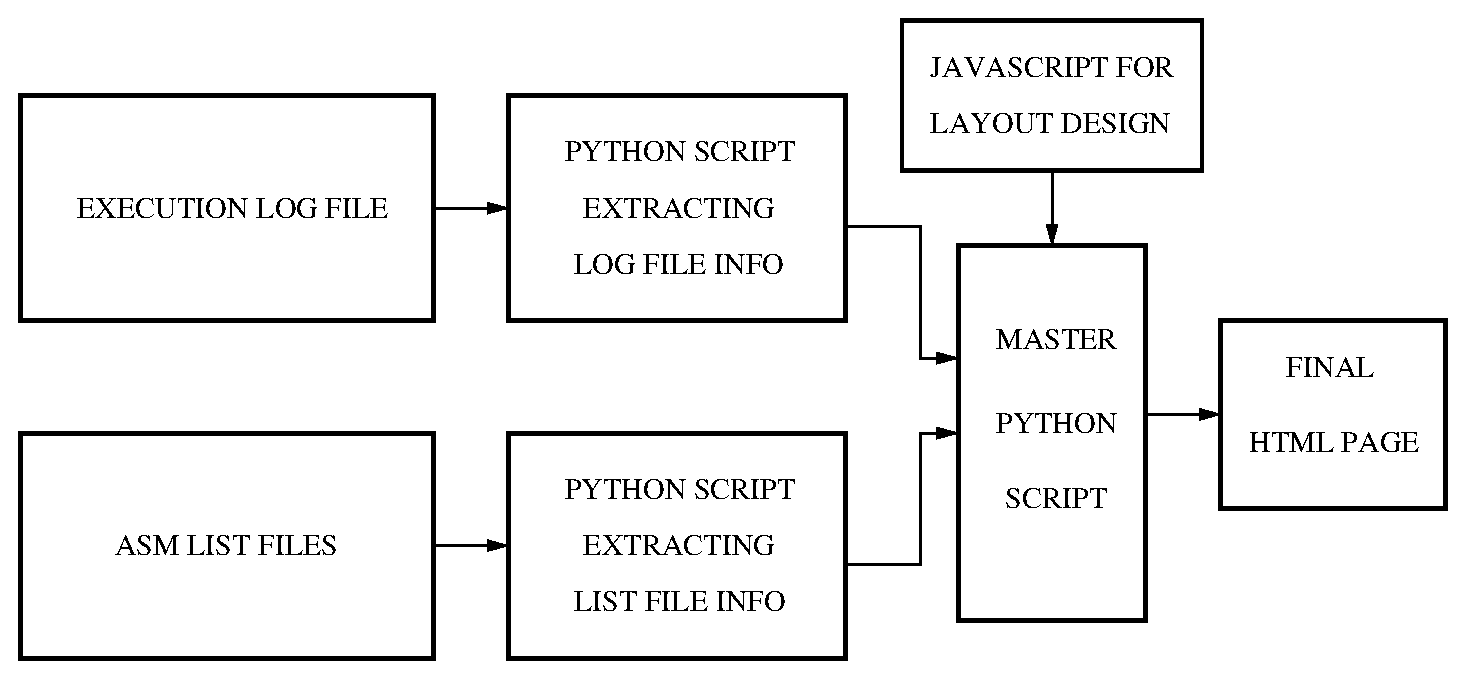
\includegraphics[scale=0.5]{./figures/gui_impl.ps}
\caption{GUI Implementation} 
\label{fig:gui_impl.eps}
\end{figure}

\figurename{\ref{fig:gui_impl.eps}} depicts information extraction and use of different scripts to achieve the same. Major implementation steps
\begin{itemize}
\item[-] Extraction of information from assembly list file and processor execution log by python script.
\item[-] Correlation of information from previous step.
\item[-] Coding generic JavaScript code for user interactions.
\item[-] Top level python program to manipulate available information and to convert it to JavaScript information. 
\item[-] The top level python program will combine the data extracted and javascript code to generate a single HTML page. 
\end{itemize}

The whole infrastructure is packaged neatly. Given execution log file and assembly list file, the top level python script generates the HTML interface web page. Different stages involved in this conversions are described in the following sections. 

\subsection {INTERFACE}
GUI is targeted to run on any browser, hence layout design is done using {\it HTML}\nomenclature{HTML}{Hyper Text Markup Language}. However for providing interactive features to the user, a much more powerful language is need along with HTML and default choice is JavaScript.

\emph {\bf JavaScript (JS)} is an interpreted computer programming language. It is  implemented as part of web browsers so that client-side scripts could react to user inputs, customize the browser, communicate asynchronously, and to filter contents being displayed. It is a multi-paradigm language, supporting object-oriented, imperative, and functional programming styles.  
In addition a style sheet language called CSS\nomenclature{CSS}{Cascading Style Sheets} is used for describing the presentation semantics (the look and formatting) of the interface page written in HTML.

%\figurename{} 
%\figurename{} 
\begin{figure}[h]
\centering
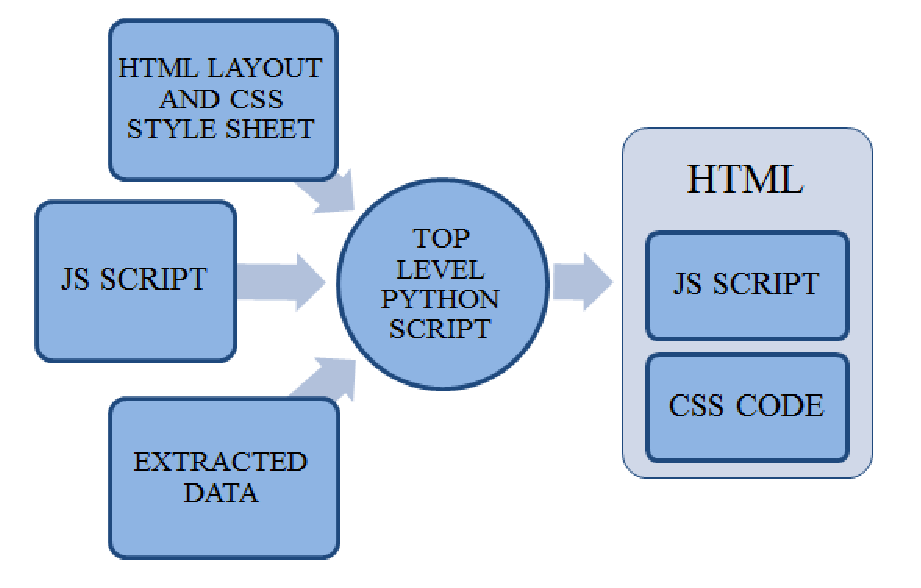
\includegraphics[scale=0.75]{./figures/html.ps}
\caption{Web Page Generation}
\label{fig:html.ps}
\end{figure}

Resultant HTML page embeds JavaScript routines and style sheets. This is done by the top level python script. \figurename{\ref{fig:html.ps}} shows a representation of information flow.


\subsection{JS DATA STRUCTURE}
All dynamic features of the interface are handled by JS\nomenclature{JS}{JavaScript} script routines. Data input to the JS is the extracted information from execution log files and list files. The top level python script converts the extracted objects into JS data array ``$dataArray[]$'' ; where each array element corresponds to an active thread. Active threads refer to active core or processor in a multiprocessor system.  

\IncMargin{1em}
\begin{algorithm}[h]
\DontPrintSemicolon
\SetKwInOut{Input}{Input}\SetKwInOut{Output}{Output} \SetKwFunction{KwFn}{CreateDataArray}
\KwFn {}
\BlankLine
\Begin{
\For {i in activeThreads}{\;
		\For {$log$ in logObj}{\;
		\If{log.Id == i}{
		Append $log \rightarrow	DataArray[i]$\;
		}
}
}
}
\caption{Creating JavaScript Object}
\end{algorithm}\DecMargin{1em}



Once the extracted information is converted to JS compatible data, the interface features can utilize this. The layout for various GUI features called windows, are designed using HTML and CSS code. All dynamic interactive features are handled by embedded JS script in HTML web page. Later sections introduces different windows available in the web page.

\section {EXTRACTION OF INFORMATION}
The first step in creating a generic debug interface is to extract relevant information and convert it to a format that could be loaded by the debug interface.

\subsection {STIMULUS}
Stimulus is written in X-86 assembly language. The engineer is expected to debug this stimulus. Each cycle in processor execution log corresponds to a particular assembly code. An assembler is used to assemble to object code, in that process each instruction is also mapped to a particular address. \figurename{\ref{impl.tex:assembler}} shows this process which also produces a list file which hold an macro expanded, loop unrolled, assembled code with corresponding address details. The configuration file defines certain random operands, segmentation, gdt, ldt, page tables to aid in assembling process. The include files contribute common routines used across different assembly stimuli.

%However, the written by the verification engineer is the unscheduled code without any memory address details. For cycle comparison with execution log, the asm test file is complied first.

\begin{figure}[h]
\centering
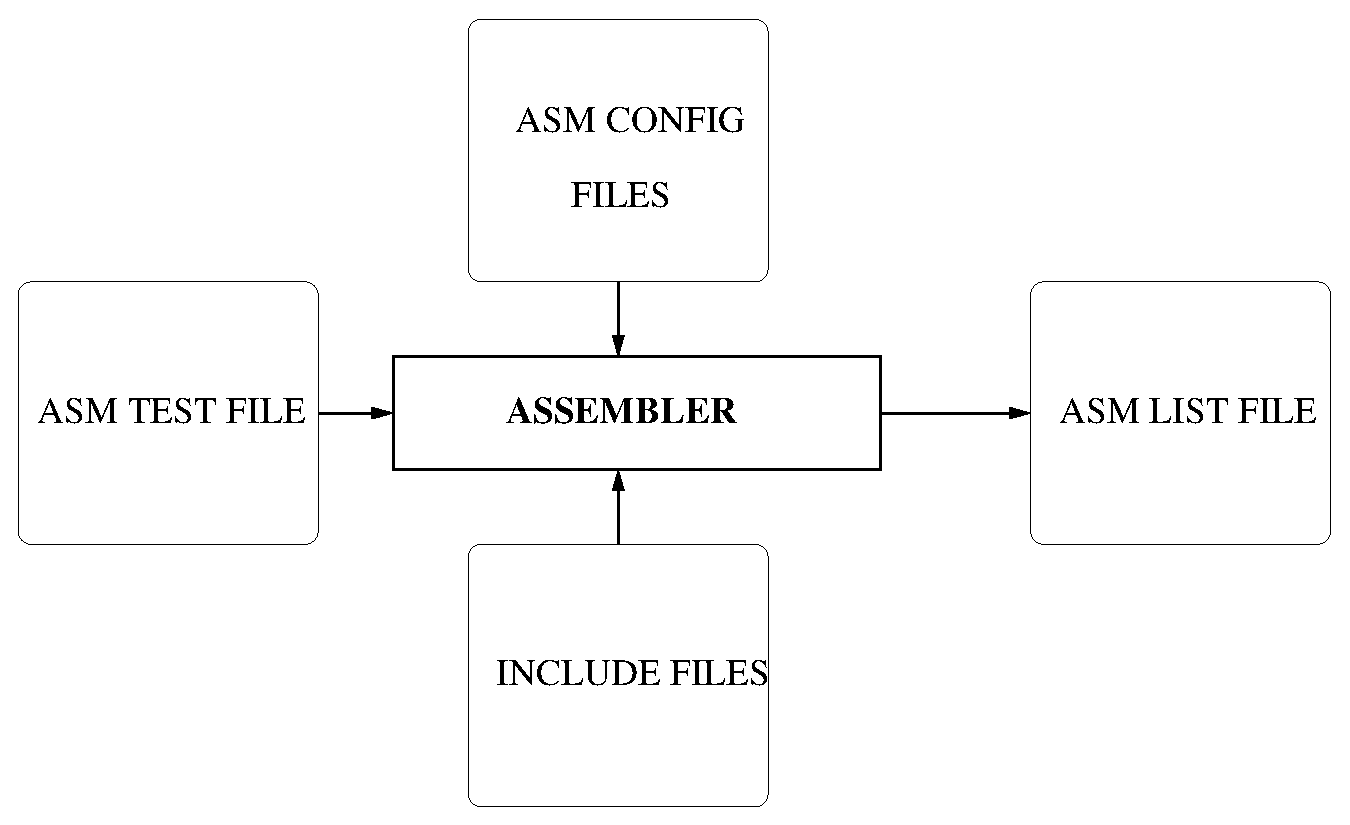
\includegraphics[scale=0.5]{./figures/asm.ps}
\caption{Assembler}
\label{impl.tex:assembler}
\end{figure}


\begin{figure}[h]
\centering
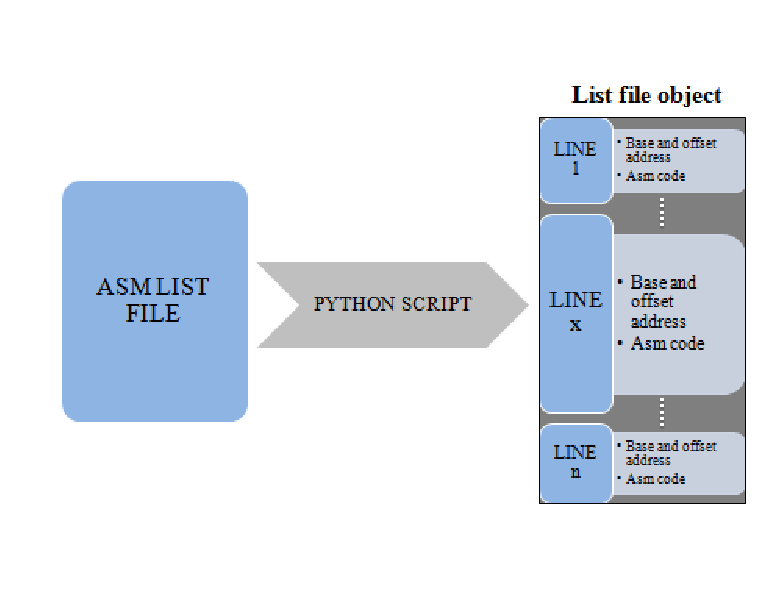
\includegraphics[scale=0.5]{./figures/list.ps}
\caption{Asm List File Extraction}
\label{impl.tex:listextr}
\end{figure}

List file holds a wealth of details including instructions, opcodes, operand, linear address, module/register configuration details etc. A {\it python} script is used to extract relevant information corresponding to each instruction line in the list file. In this project, the following information is extracted for each instruction from the  list file:
\begin{itemize}
	\item[-] Base and offset address value
	\item[-] Instruction line number
	\item[-] The assembly code
\end{itemize}

The {\it python} script internally contains a data structure of list objects, which helps in adding features to the script with ease (\figurename{\ref{impl.tex:listextr}}). 

\subsection {EXECUTION LOG}
Execution log file contains instruction by instruction execution details from simulation. It also includes register states, thread details, flag values and other details which help in tracing out the cause of failure. As explained in previous chapters, debugging require detail traversal through this log file. 

Details in the log file with reference to each cycle is required to be extracted. {\it Python} script is used to extract these informations as well and a comprehensive data structure is created. The data structure objects contain properties corresponding to major operations and register values. Thread details are handled as separate data structures as it aids processing thread-wise informations. Following properties are extracted from execution log file for every execution event

%Figure x shows how the script will read the input execution log file and generate log file objects.

\begin{itemize}
 \item[-]  Thread number
 \item[-]  Mode of operation
 \item[-]  Cycle number
 \item[-]  Linear address
 \item[-]  Memory write, Memory read, I/O write/read, Code read
 \item[-]  Branch target (linear address)
 \item[-]  New values of registers, if modified
\end{itemize}


\subsection {INFORMATION CORRELATION}

Once both the input files are processed, next step is to correlate assembly with execution log. A {\it python} script can accomplish this by correlating respective data structures based on linear addresses. As x86 architecture follows segmented memory model along with paging, address translation is required for generating the linear/physical address\cite{SS:AMD64-V2}. Linear address is calculated as
\\
\centerline{Linear address = Base address + Offset value}
\\


%\vspace{1.5cm}

\IncMargin{1em}
\begin{algorithm}[h]
\DontPrintSemicolon
\SetKwInOut{Input}{Input}\SetKwInOut{Output}{Output} \SetKwFunction{KwFn}{CreateDataArray}

\Input{list file objects$\rightarrow listObj[]$, log file object$\rightarrow logObj[]$}
\BlankLine
Start: \;
\For {each object $list$ in listObj}{\;
		list.address = list.Base + list.Offset\;
	}
\For {each object $log$ in logObj}{\;
	set count = 0\;
	\For {each object $list$ in listObj}{\;
	 \If{$log.address == list.address$}{
		Append each $list$.property $\rightarrow$ $log$.property\; \tcp{$log$ properties are lineNo, opcode and address}\label{cmt}
		count = 1;
		break loop\;
	}
	}
	\If{count == 0}{
	assert: $"no address match"$
	}
}
End \;
\caption{Combining List and Log File Information}
\label{algo:impl:cllf}
\end{algorithm}\DecMargin{1em}

%\vspace{1.5cm}

For each object of execution log, the corresponding list file object could be found based on linear address value. Once found, both are cross-linked to aid further processing. The algorithm employed in this search is depicted in Algorithm~\ref{algo:impl:cllf}. Data extraction is complete with this linkage and the result is execution log objects linked to corresponding assembly objects.

\section {GUI FEATURES}

\subsection {EXECUTION FLOW GRAPH}
Main feature of debug interface is the graph showing the execution flow of the code. It is obtained by plotting asm list file line numbers against the execution cycle during which it is executed. All the active threads have different graphs which are tabbed. Hovering the mouse over any execution point on the graph will display $X$ and $Y$ axis values. Features include zoom-in, zoom-out of plot. Double click at any point is featured to zoom-out completely. On clicking on any execution point, selects the point and syncronizes data across windows. Proximity click feature helps in automatically choosing nearest execution point for further analysis.
 
The flow graph also features customisable selection of specific processor operations out of Branching, Memory Write, Memory Read, Code Read. This helps in filtering redundant execution points those may not be of interest to the engineer. Each distinct processor operation could be distinguished by color coding.   

\subsubsection {IMPLEMENTATION}

Execution flow graph is created with Dygraph JavaScript Visualization Library\cite{http:dygraphs}. The library provides inbuilt functions that enable zooming, x-y axis value display and point ``{\it onClick}'' callbacks. {\it onClick CallBack()} function is called whenever an execution point on Dygraph is clicked. The function has been extended to activate other windows and to synchronize components across windows.

Graph could be built by providing independent axis values followed by depended axis values. For each thread, a different graph is generated but layered out on different HTML tabs. The x-axis is cycle number and y-axis is the list file line number. Algorithm~\ref{algo:impl:ceg} shows the pseudo-code used in building the graph in our application.

\IncMargin{1em}
\begin{algorithm}[h]
\DontPrintSemicolon
\SetKwInOut{Input}{Input}\SetKwInOut{Output}{Output} \SetKwFunction{KwFn}{CreateGraph}
\KwFn{}
\BlankLine
\Begin{
\For {each i in activeThread}{\;
\For {each element in dataArray[i]}{\;
	Dygraph[i] $\leftarrow [element.cycleNo , element.lineNo]$\;
	}
}
}
\caption{Creating Execution Graph}
\label{algo:impl:ceg}
\end{algorithm}\DecMargin{1em}

\subsection {REGISTER WATCH WINDOW}
\label{sec:impl:rww}
Register window is used in displaying instantaneous register values at any execution point. Under the hood, thread based register values are maintained separately, as it aids user switching back and forth between threads of execution without loosing data on each thread. At any instant the register window holds the values of {\it selected} execution point. Selection could be changed by simply clicking on a different execution point. Register window provides values of following registers to the user:
\begin{itemize}
	\item[-] 64 bit general purpose registers (RAX, RBX, RCX etc)
	\item[-] RFLAG (64 bit)
	\item[-] Instruction Pointer (RIP)
	\item[-] Stack Pointer (RSP)
\end{itemize}

Another important feature provided by register window is a comparison of register values between two different execution points. It highlights differences in register values with different colours, to capture user's attention with ease. The difference is between {\it reference execution point} and {\it selected execution point}. {\it Reference execution point} is chosen by the {\it set~marker} button.

\subsubsection{IMPLEMENTATION}

The values contained in register window is updated when a different execution point is selected in the execution flow graph. This event also triggers comparison of current values with the reference point. Algorithm~\ref{algo:impl:crw} lists the pseudo-code used in updating register window values.

\IncMargin{1em}
\begin{algorithm}[h]
\DontPrintSemicolon
\SetKwInOut{Input}{Input}\SetKwInOut{Output}{Output} \SetKwFunction{KwFn}{pointonClickCallBack}
\KwFn{element}
\BlankLine
\Begin{
\For {each reg in RegisterSet}{
regRow$[reg]$ $\leftarrow$ element.$[reg]$ \;
	\If{(element.$[reg]$ != referenceRow.$[reg]$)}{\;
		$Highlight  regRow $ \;
	}
}
}
\caption{Creating Register Window}
\label{algo:impl:crw}
\end{algorithm}\DecMargin{1em}

\subsection {INSTRUCTION WINDOW}

Instruction window lists the assembly code corresponding to the selected execution point. Context around the assembly code is also displayed to aid debug. This window is also updated when a different execution point is selected in execution graph. The window highlights assembly code for visual attention of the user.

\subsubsection{IMPLEMENTATION}

The pseudo-code used to update values in this window is shown in Algorithm~\ref{algo:impl:ciel}.

\IncMargin{1em}
\begin{algorithm}[h]
\DontPrintSemicolon
\SetKwInOut{Input}{Input}\SetKwInOut{Output}{Output} \SetKwFunction{KwFn}{onClickCallBack}
\KwFn{element}{;\
\BlankLine
\Begin{
\For {each item from element-50 to element+50}{\;
	Add $item.opcode \rightarrow$ InstructionWindow\;
	}

Add $item.logInfo \rightarrow$ ExecutionLogWindow\;
}
}
\caption{Creating Instruction and Execution Log Window}
\label{algo:impl:ciel}
\end{algorithm}\DecMargin{1em}

\subsection {EXECUTION LOG WINDOW}

In addition to the instruction and register information, the relevant processor execution log in its actuality, would be useful to the user as it contains different information that may not be presented by the debug interface. Having this information readily accessible to user also assures the user that the data extracted through processing by different scripts is indeed correct. Internally these informations are stored as a JavaScript object ``{\it logInfo}''.

%Implementation of Execution log window is given in algorithm x along with instruction window.

\subsection{MARKERS}
As it was discussed in Section~\ref{sec:impl:rww}, markers are used to ``mark'' reference execution point through a ``Set Marker'' button. Button ``Clear Marker'' could  be used to clear the marker.

\subsubsection{IMPLEMENTATION}

Set and Clear buttons are implemented using HTML form's callback feature. A {\it JavaScript} variable is used to store the reference execution point.


 

%%%%%%%%%%%%%%%%%%%%%%%%%%%%%%%%%%%%%%% GUI FEATURES %%%%%%%%%%%%%%%%%%%%%%%%%%%%%%%%%%%%%%%%%%%%%%%
%\newpage
%\chapter{GUI FEATURES}
\label{chap:GUI_features.tex}
%\addtocontents{toc}{\protect\setcounter{tocdepth}{0}}

The master Python script reads all the extracted information from the log files and the list files. This script finally generates a single HTML page for the interface. The interface mainly features:


\section {EXECUTION FLOW GRAPH}

Main feature of the web page is the graph showing the execution flow of the code. Here asm list file line numbers are plotted against the cycle during which it is executed. All the active threads have different graphs which are tabbed. Hovering the mouse over any point on the graph will display x and y axis values. 
 
This zoom enabled data graphs also provides onclick selection of specific operations e.g: Branching, Memory Write, Memory Read, Code Read etc, which will display the instances of selected operation. Each operation is distinguished by its color.   


\section {REGISTER WATCH WINDOW}

Register window capture and display updated register values at a specific instance. Each thread holds its own copy of registers/flags. A selection of point on the execution flow graph will update the register window with values at that instant in the selected thread. Values of following registers and flags are provided to the user:

\begin{itemize}
	\item[-] 64 bit general purpose registers (RAX, RBX, RCX etc)
	\item[-] RFLAG (64 bit)
	\item[-] Instruction Pointer (RIP)
	\item[-] Stack Pointer (RSP)
\end{itemize}

Another feature provided by register window is comparison between register values at two different instances that is between a reference point set by Set Marker button and current selection. 


\section {INSTRUCTION WINDOW}

Instruction window give the asm file lines. A selection in execution graph will be reflected in this window by highlighting the asm file instruction corresponding to the selected point. Also the context of the selected line that is its preceding and succeeding instructions are also available in this window.

\section {EXECUTION LOG WINDOW}

In addition to the instruction and register information, all the processor execution log information regarding the selected instruction is also provided through execution log window.

\section{SET AND CLEAR MARKER}
These two options allow setting or removing a reference point with which current register values are compared against.

 


%%%%%%%%%%%%%%%%%%%%%%%%%%%%%%%%%%%%%% RESULT: GUI %%%%%%%%%%%%%%%%%%%%%%%%%%%%%%%%%%%%%%%%%%%%%%%
\newpage
\chapter{RESULTS: GRAPHIC USER INTERFACE}
\label{chap:GUI_results.tex}
\addtocontents{toc}{\protect\setcounter{tocdepth}{1}}
The final GUI is a self contained {\it HTML} page generated by the master {\it Phython} script which derives informations from assembly list files and execution log files. The generated {\it .html} file could be viewed by any standard web browser (like Internet Explorer, Firefox, Chrome) those support {\it JavaScript}. Care is taken that this generated {\it HTML} is devoid of dependencies and thus it enables interactive debug from remote locations. The only requirement for the user is network connectivity to receive the html page. The following figures shows various windows of final GUI.
\section {EXECUTION FLOW GRAPH}
%\figurename{} 
\begin{figure}[h]
\centering
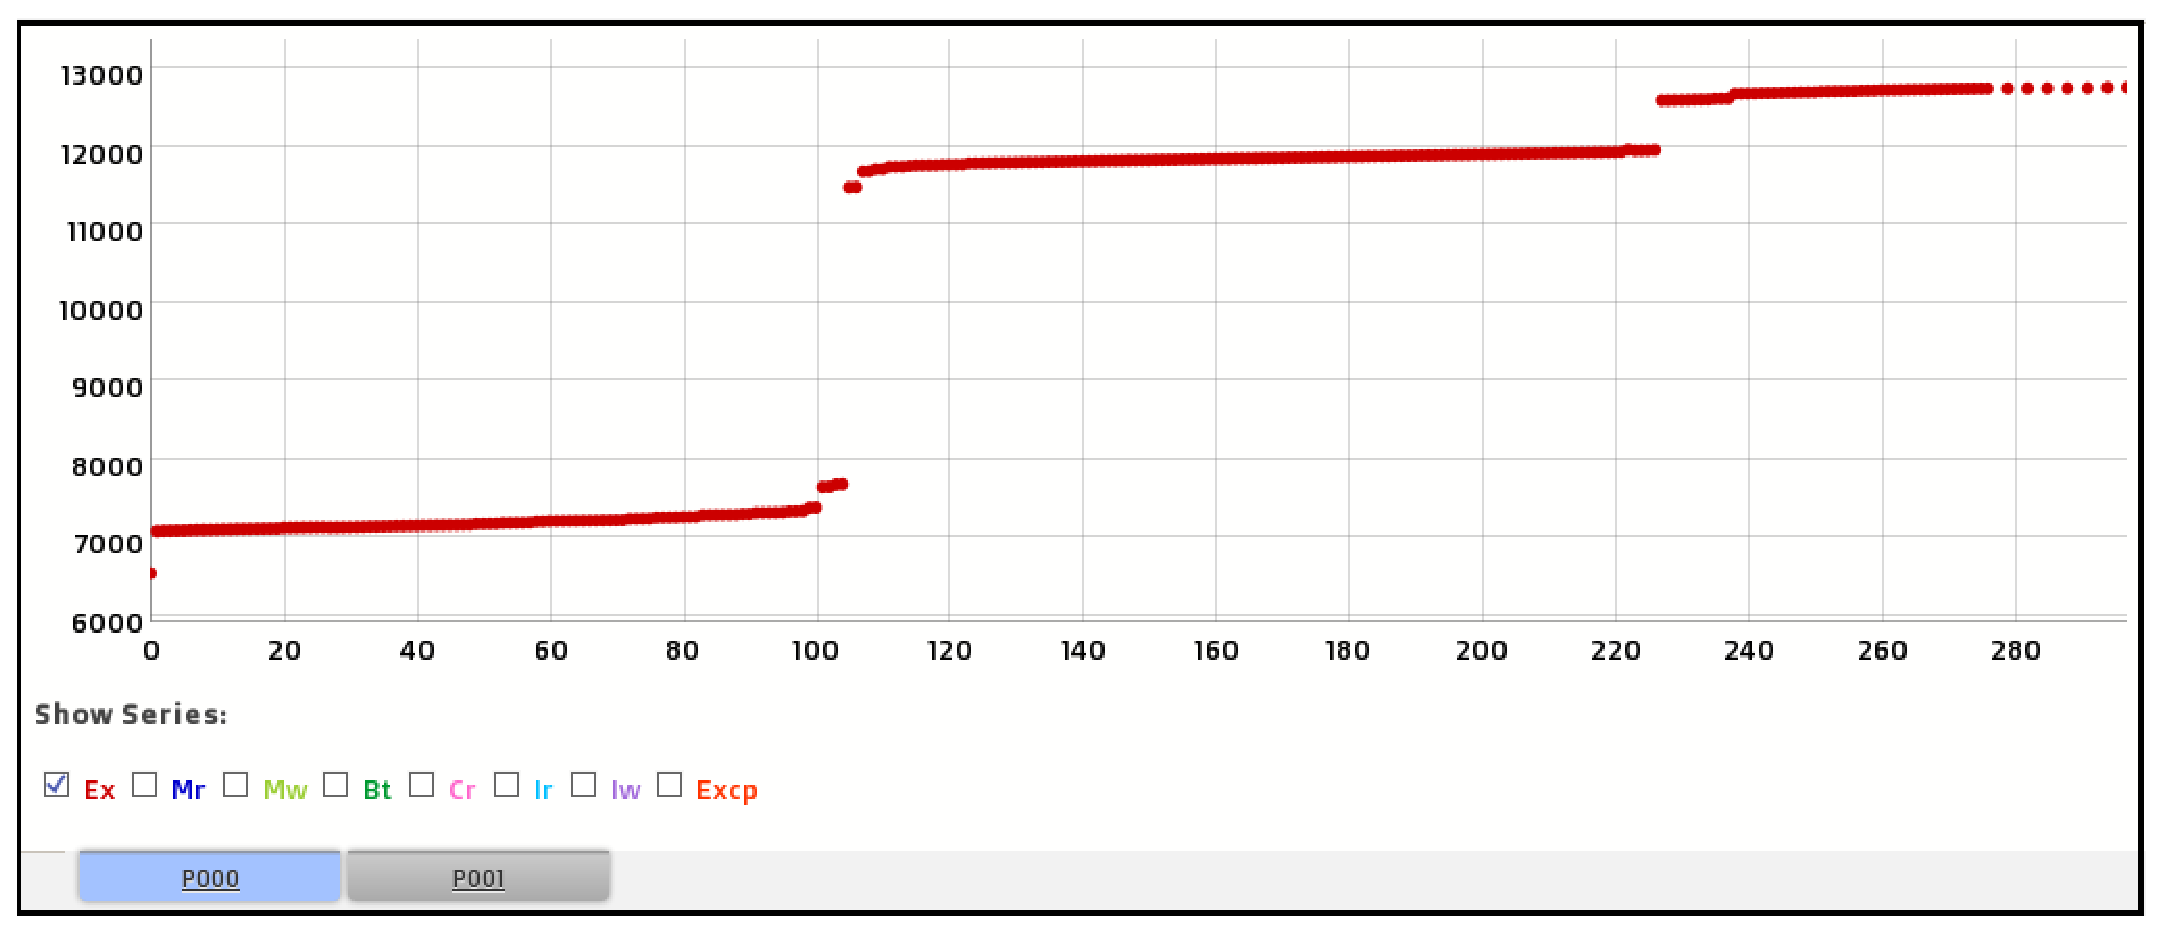
\includegraphics[width=6in]{./figures/gui_graph1.eps}
\caption{Execution Flow Graph}
\label{fig:gui_graph1.eps}
\end{figure}
%\end{tabular}
%\figurename{} 

\begin{figure}[h]
\centering
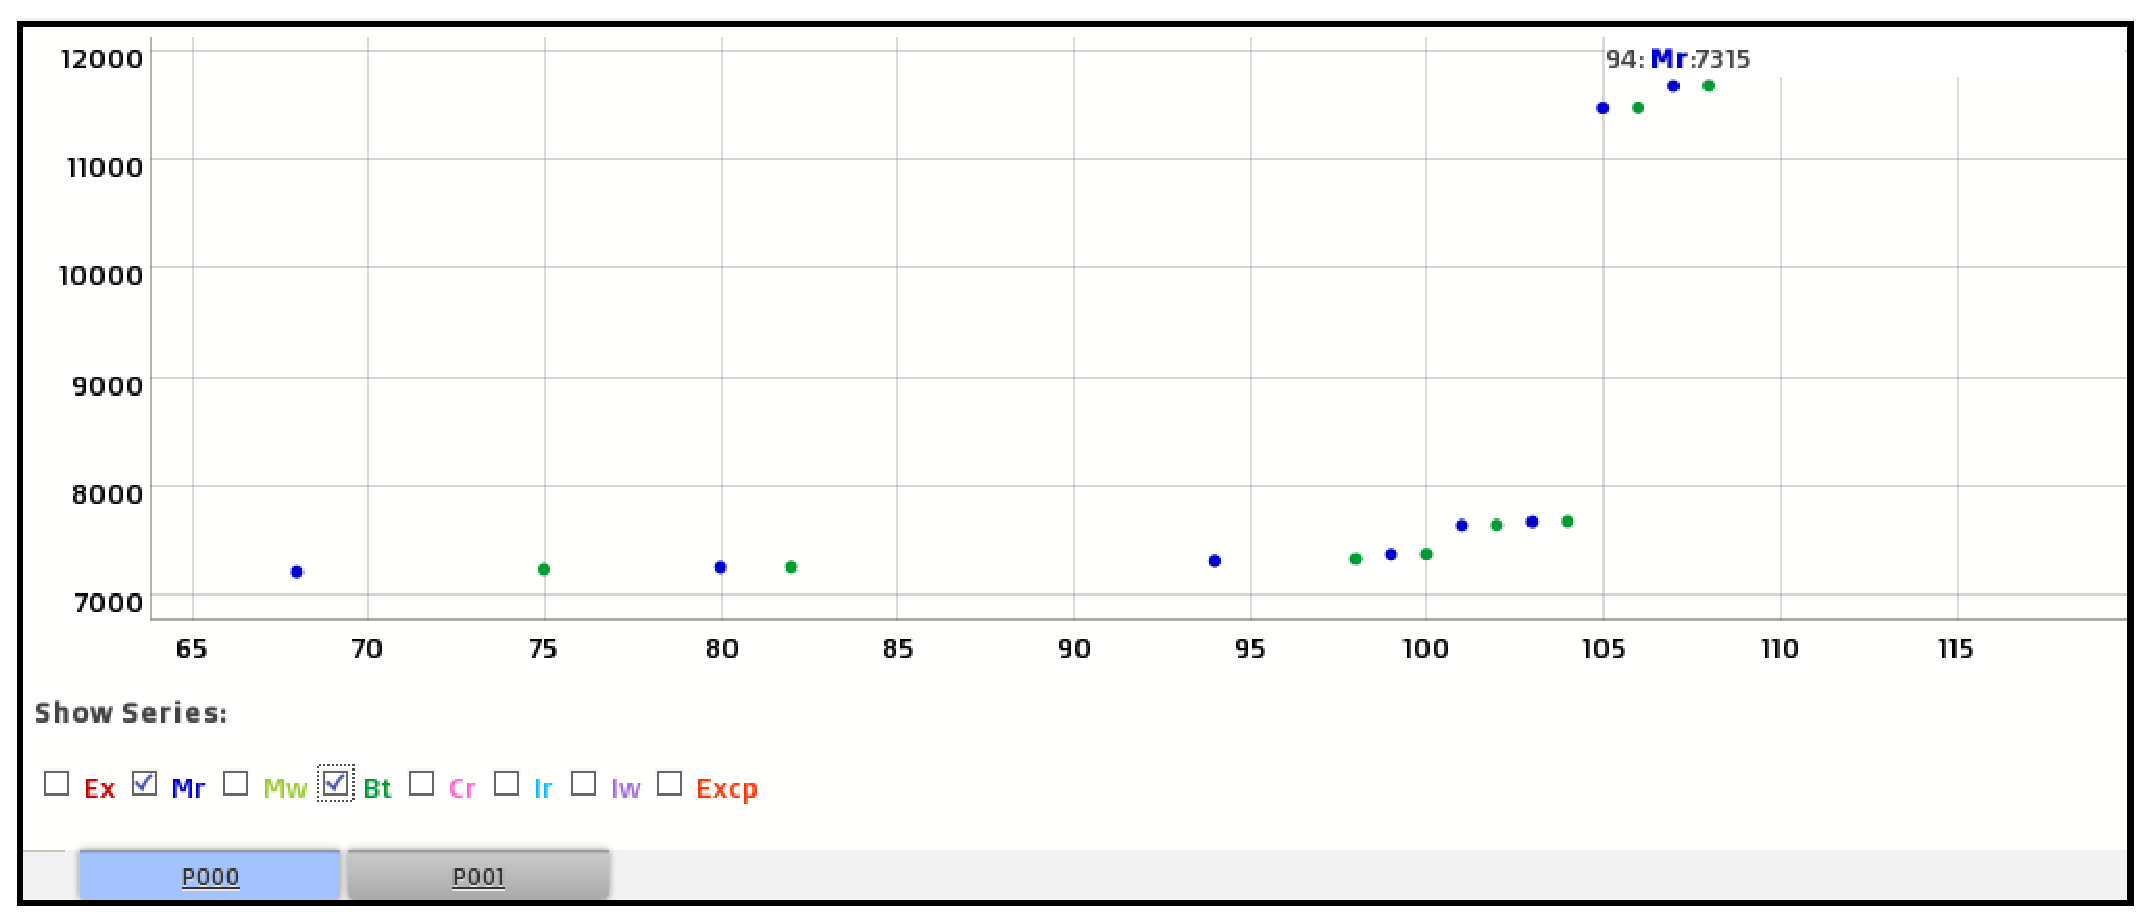
\includegraphics[width=6in]{./figures/gui_graph2.eps}
\caption{Execution Graph With Branching and Memory Writes}
\label{fig:gui_graph2.eps}
\end{figure}
%\end{tabular}
%\figurename{} 

~\figurename~{\ref{fig:gui_graph1.eps}} shows the main execution flow graph for selected active thread.  
~\figurename~{\ref{fig:gui_graph2.eps}} highlights execution points in which memory writes and branch operation occurs. The appropriate checkboxes towards bottom indicates the selection made. Note that thread {\it P000} is the active tab and inactive tab for {\it P001} is layered below it and could be selected.
\section {REGISTER WATCH WINDOW}
\begin{figure}[h]
\centering
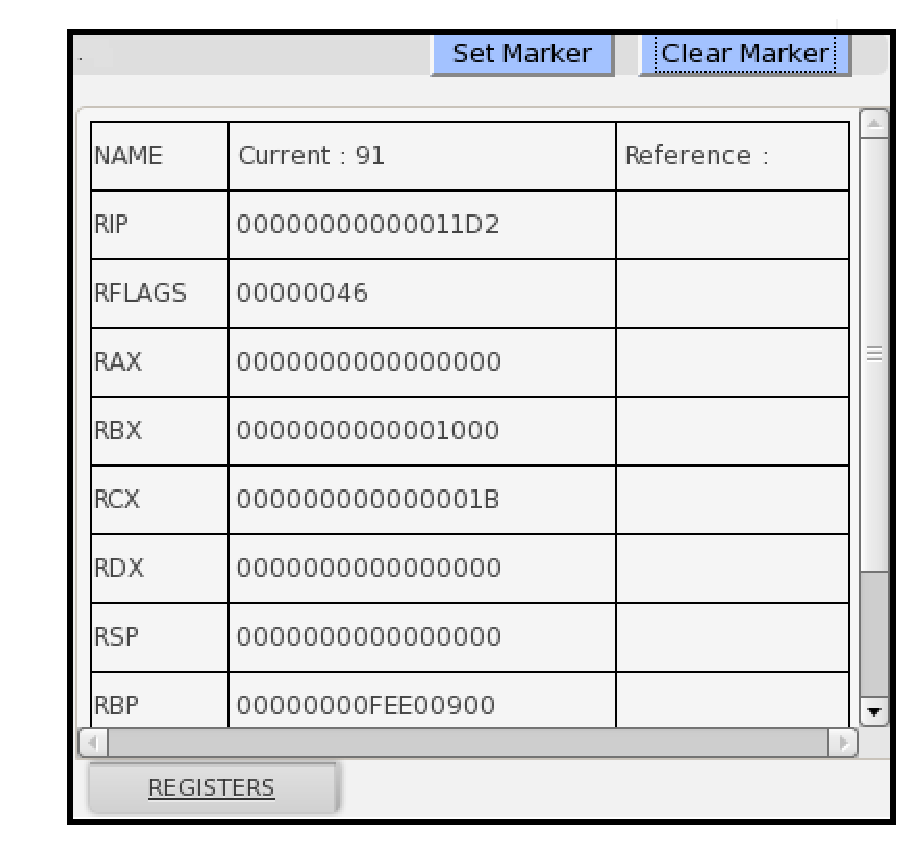
\includegraphics[width=4in, height=2in]{./figures/gui_reg1.eps}
\caption{Register Watch Window}
\label{fig:gui_reg1.eps}
\end{figure}
~\figurename~{\ref{fig:gui_reg1.eps}} is the register window. It could be observed that register values corresponding to selected execution point {\it cycle 91} is shown in {\it current selection} column. {\it Set~Marker} and {\it Clear~Marker} buttons could also be observed in the snapshot.
%\end{tabular}
\begin{figure}[h]
\centering
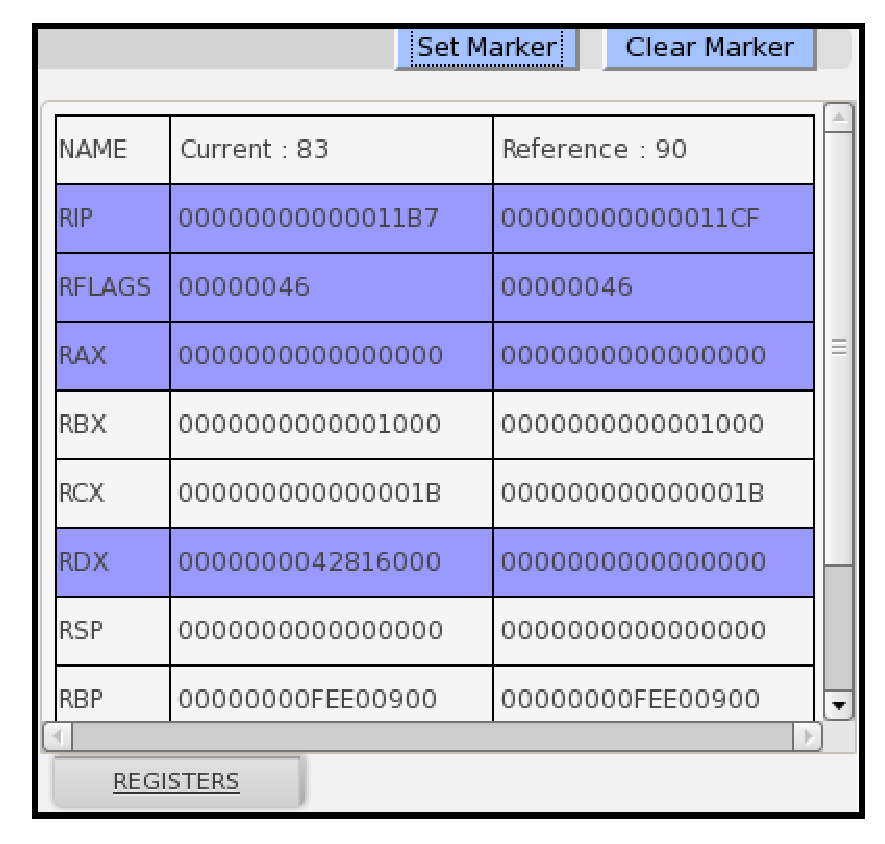
\includegraphics[width=4in, height=2in]{./figures/gui_reg2.eps}
\caption{Register Value Comparison}
\label{fig:gui_reg2.eps}
\end{figure}
%\end{tabular}
~\figurename~{\ref{fig:gui_reg2.eps}} shows the comparison of register states at two different points. Differences are highlighted.
\section {INSTRUCTION WINDOW}
\begin{figure}[h]
\centering
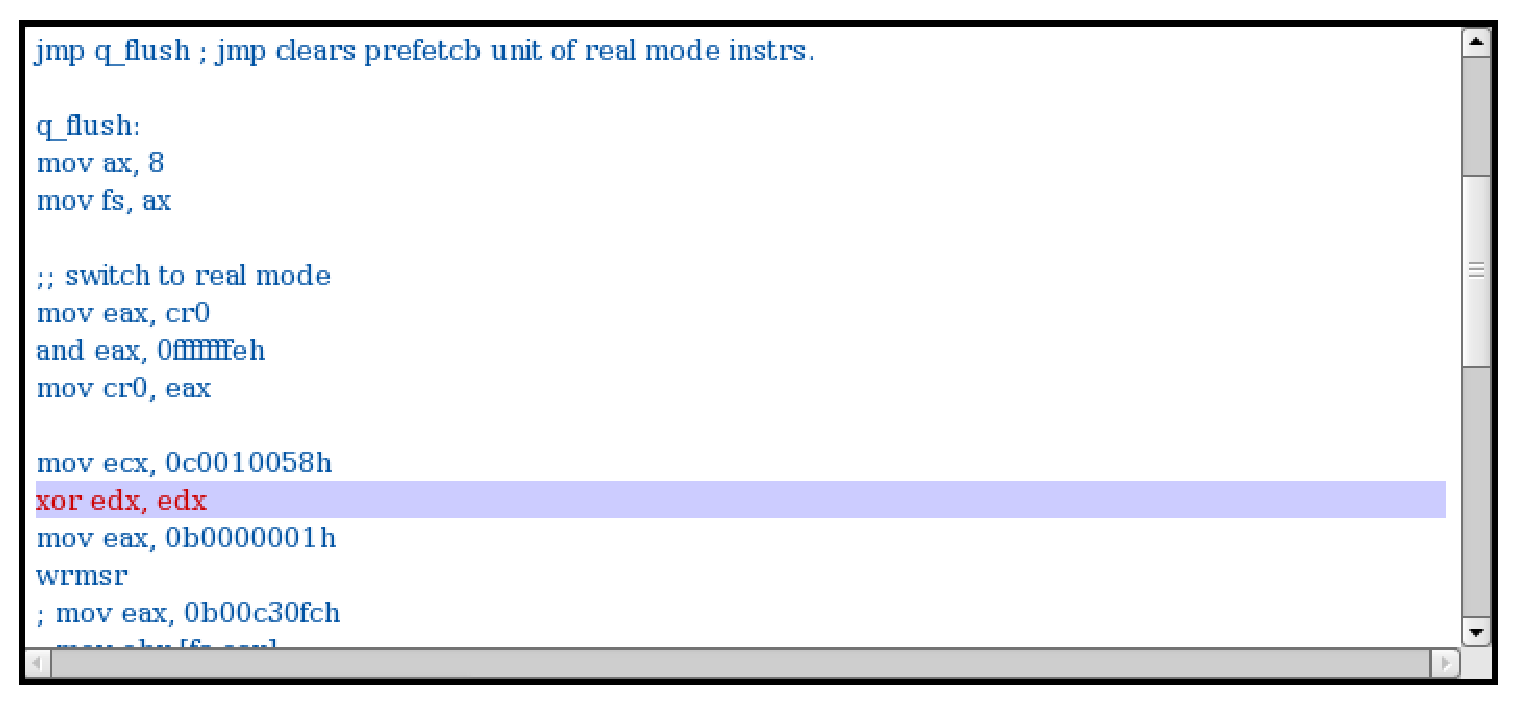
\includegraphics[width=5in, height=3in]{./figures/gui_asm.eps}
\caption{Instruction Window}
\label{fig:gui_asm.eps}
\end{figure}
%\end{tabular}
~\figurename~{\ref{fig:gui_asm.eps}} is the instruction window. The instruction window could be seen highlighting the assembly along with its context, corresponding to the selected execution point.


 

%%%%%%%%%%%%%%%%%%%%%%%%%%%%%%%%%%%%%% CONCLUSION %%%%%%%%%%%%%%%%%%%%%%%%%%%%%%%%%%%%%%%%%%%%%%%
\newpage
\chapter{CONCLUSION}
\label{chap:GUI_conclusion}

An interactive off-line graphical user interface was designed and developed. The interface is completely web based and achieves primary goals of off-line debug. The interface contains all relevant information from processor execution log and assembly list files commonly needed for debug. Further debug if required, could be accomplised by traditional methods.

Execution graph helps in analysis of various operations like branching, exception, read/write etc and also to navigate through processor execution with ease. The graph presents thread-wise informations seperately, making tracing and navigation easy. The register window provides comparison between registers and flag values at two different execution cycle which helps in tracing a wrong value written into register or flag. Instruction window and execution log window provide common information necessary for debug.

\paragraph{Potential for future work:} The project demonstrates that web-based technologies like {\it html, JavaScript, CSS} are effective in enabling interactive remote debug. There is larger scope for this work in future as it gets adopted by different teams. New debug features like break points, cache containers, address filters among others could be needed in the future. Care has been taken to preserve design modularity, so that such fetures could  be added in the future.




%%%%%%%%%%%%%%%%%%%%%%%%%%%%%%%%%%%%%% PART II : GATESIM %%%%%%%%%%%%%%%%%%%%%%%%%%%%%%%%%%%%%%%%%%%%%%%%%%
\part{}

%%%%%%%%%%%%%%%%%%%%%%%%%%%%%%%%%%%%%% INTRODUCTION %%%%%%%%%%%%%%%%%%%%%%%%%%%%%%%%%%%%%%%%%%%%%%%
\newpage
\chapter{INTRODUCTION}
%\section{Background}
%\section{Purpose/Motivation}
%\section{Approach}
%\section{Main Contributions}
%\section{Organization of thesis}

Functional verification of a design is the task of verifying that the logic design conforms to specification and ensures functional correctness of the design.  With the rapid increase in design complexity and size, this phase of circuit design has become the most crucial and resource-intensive. It is widely accepted that more than 70 percent of design efforts is spend on verification and with the advancement in silicon technology and adoption of complex SoC designs; this situation is only projected to get worse in future. 

Verification is done at different abstraction levels. Two main abstraction levels from verification point of view are RTL and gate level. RTL enables relatively easier management of complex designs and has less verification time requirements compared to gate or netlist level. However it cannot overcome the need for verification at netlist level as each level is required for specific type of verification. While RTL verification is apt for functional validation or architectural analysis, more detailed analysis like timing, power etc require detailed models of lower levels. Another important challenge is ensuring the functional equality of models at different abstraction level.  

 Traditionally simulation based verification has be used as the primary approach for verification at both RTL as well as gate level.  But with very complex designs, this approach has become inefficient in finding subtle design bugs. Also at gate level, simulation based verification takes rather too much time that an exhaustive verification is impossible. On the other hand, formal verification tools have gained popularity since it can mathematically prove or disprove the design validity. These mathematical methods require less manual effort than simulation based verification and hence a lot faster. However these mathematical models cannot comprehend all kind of complexities that could occur in the design and it is very much clear that this alone can solve all issues. Rather a mix of simulation and formal verification methods are practiced to ensure all corner cases are covered. 


\section{GATE LEVEL SIMULATION}

In spite of advancement in formal verification techniques, mainly LEC and STA, gatesims still play crucial role in gate level verification.   Having gatesim in the design low means there is a necessity of early planning for this. It has to pass through various stages before sign off and helps in functional as well as timing analysis. The setup for gate level simulation starts right after the prelim netlist is released and will extend till simulation of post layout netlist.  

Even though gatesims help in resolving many issues, this phase of verification is considered as a "{\it necessary evil}" by engineers. This is mainly because gate level simulation is inherently very slow and also finding an optimal list of test cases to effectively utilize gatesim to find functional and timing errors is hard. Debugging is a very tedious process at gate level and the long run time makes rerun for debug hard and ultimately affect the final time-to-market.  

Various approaches have been adopted over the years for gate level simulation with each method trying to improve simulation performance and ease of debug. Since generally netlists are Verilog based, test environments similar to RTL can be used to simulate the net list. Alternative way is to have the same test vectors generated for RTL simulation used as stimulus for netlist simulation. This can be in two ways: one having the RTL run in parallel with gatesim, and second way is to capture the test vectors generated for RTL simulation and applying it as stimulus for gate. The first case is called a co simulation approach and the second is dual-simulation or sim after sim. Each method comes with its own set of pros and cons. Usually there are time, memory, ease of debug, testbench complexity tradeoffs while choosing any particular method for gatesim. This thesis analyzes the advantage and disadvantage of past and present gatesim methodologies and  proposes a new improved sim after sim or dual simulation approach to gatesims. 



\section{ORGANIZATION OF THE THESIS}
The organization of this project report is as follows:\\
\noindent 
{\bf Chapter}~\ref{chap:gate_intro.tex} -{\it Gate Level Simulation} explains the relevance, advantages and limitations of gate level simulation.\\
{\bf Chapter}~\ref{chap:methodologies.tex} -{\it Gatesim Methodologies} briefly explains various approaches used for gatesim and their advantages and disadvantages.\\
{\bf Chapter}~\ref{chap:dualsim.tex} -{\it Improved Dual-Sim Approach To Gatesim} describes the implementation and flow of proposed dual sim approach .\\
{\bf Chapter}~\ref{chap:results.tex} -{\it Results} gives comparison of simulation performance and memory utilization of current approach and proposed approach.\\
%{\bf Chapter}~\ref{chap:GUI_results.tex} show the GUI windows and    .\\
%{\bf Chapter}~\ref{chap:conclusion} discusses the various 
%conclusion drawn from the results and the scope for future work.

 

%%%%%%%%%%%%%%%%%%%%%%%%%%%%%%%%%%%%%% GATE LEVEL SIMULATION %%%%%%%%%%%%%%%%%%%%%%%%%%%%%%%%%%%%%%%%%%%%%%%
\newpage
\chapter{GATE LEVEL SIMULATION}
\label{chap:gate_intro.tex}

In a typical VLSI design flow for verification, the first step after RTL level model of the design availabilty is writing behavioral test bench for functional verification. The functionally verified RTL goes through design synthesis during which it is mapped into low level design components in terms of primitives or logic gates. Synthesis is mostly an automated process using a ``{\it synthesizer}'' tool that converts RTL-level design source code into corresponding gate-level netlist mappings. This netlist is also called the pre-layout netlist.

The pre-layout netlist that was obtained from synthesis is then fed into a layout tool which maps the gate primities to silicon structures such as channels, gates, vias, etc. During this process certain modifications are done on netlist but it should not alter its functionality to its corresponding RTL. To validate this, another netlist called the post-layout netlist is generated back from the layed-out silicon structures by the layout tool itself. Validation is made by running LEC tool over both pre-layout and post-layout netlists or between post-layout netlist and RTL.

Though it would be ideal to use post-layout netlist for the purpose of gatesims, it would be too late in the design process. So work on gatesims starts with pre-layout netlist and progresses to post-layout netlist as it becomes available. ~\figurename{~\ref{fig:vlsi_design.ps}} depicts progress of gatesim with respect to other design flows.

%\figurename{} 
\begin{figure}[H]
\centering
\includegraphics[width=3.5in]{./figures/vlsi_design.ps}
\caption{Design Flow}
\label{fig:vlsi_design.ps}
\end{figure}
Gate Level Simulation or Gatesim focuses on verifying the post layout netlist of the design. Gatesims are historically present from the days when designs were done with gates rather than at RTL abstraction. Verification with gates is a huge confidence builder before manufacturing of actual silicon as they are also thought to complement and reassure results obtained from formal flow.


\section {NEED FOR GATESIM}
Gatesims are particularly effective for the following verification
\begin{itemize}
	\item[-]Power-up, reset propagation and initialization of the design
%% Naren:isitso?:	\item[-]The RTL written is synthesizable.
	\item[-]DFT structures those are absent in RTL and added during or after synthesis
	\item[-]non-resettable or un-initialized components such as memories
%% Naren:what?:	\item[-]The netlist passes all the critical test scenarios.
	\item[-]Power related circuits those are absent in RTL
	\item[-]Power switching verification
	\item[-]Dynamic power estimation
	\item[-]Validation of pessimistic behaviour of X-propagation in RTL simulation
	\item[-]Asynchronous interfaces those are false-paths in STA
	\item[-]Synchroniser logic and clock domain crossing verification
	\item[-]Analog-circuit and digital circuit co-verification
\end{itemize}

Finally, Gatesim is a great confidence-booster in ensuring the high quality of the netlist. It lowers the risk of finding design, methodology or process issues in silicon.




\section{LIMITATIONS OF LEC AND STA}

Gatesims are targetted on post-layout netlist and that is almost clean of RTL bugs. The netlist also passes through couple of important verification steps such as Logic Equivalence Check (LEC) and Static Timing Analysis (STA), before it is targeted for Gatesims.

\emph {\bf LEC}: Logic Equivalence Check (LEC) is a formal verification tool that compares a reference design against a derived design to prove equivalence or to report differences.  LEC does not require test patterns. Instead, LEC uses Boolean arithmetic techniques to prove equivalence between two design descriptions\cite{ieee:boolean}. Although LEC uses sophisticated formal algorithms to identify, map, and compare nodes in the netlists, the complexity is hidden from the user\cite{lec}. %meera: what's this: [ieee] @naren: updated with cite for ieee page..

\emph {\bf STA}: Static Timing Analysis does a input-independent timing analysis of the gate level netlist. It asserts if the circuit could operate flawless without timing issues. It computes the worst-case behaviour of the circuit, over all possible manufacturing variables. STA tools are at ease in handling a complex design with huge number of paths as they consider one path at a time (whether they are real or potential false paths). 



These formal static verification techniques are much faster and evolved than simulation based methods. However these verification methodologies, in spite of advancements in tools, cannot cover all verification requirements on netlist. In addtition to reassuring results obtained by formal methods, gatesim helps in filling up the gaps left by these methods. 

Limitations of LEC, which could be covered by Gatesims are:
\begin{itemize}
	\item Limitation of Static Equivalence Checking tools to catch all X-propagation or X-generation issues.
	\item Two-state methodologies can miss RTl-versus-netlist simulation and RTL-versus-RTL simulation differences.
	\item Incorrect mapping issues due to naming at sub-block level which can result in false pass. This will not be reported at the sub-block level LEC, but Gatesims can flag such incorrect connectivity.
\end{itemize}

Limitations of STA, which could be covered by Gatesims are:
\begin{itemize}
	\item \emph{\bf X-propogation:} STA deals only with logic domain of logic-0 and logic-1. There could be many sources of indeterministic states in the design such as uninitialized flops, output of memories, synchronisers, etc. Such indeterministic state value ($X$), could propagate through and cause failure of operation. Gatesim acurately models this behaviour and but STA does not.
	\item \emph{\bf Asynchronous Interfaces:} STA ignores certain asynchronous paths called as ``false paths'', like with analog blocks or primary IO's. And hence, STA cannot verify timing between digital and analog blocks whereous Gatesims could.
	\item \emph{\bf Reset sequence:} Verifying that all flip-flops resets into their required logical value. STA cannot check this as certain declarations such as initial values on signal are not synthesizable and are verified only during simulation.
	\item \emph{\bf Asynchronous clock-domain crossings:} STA does not check if the indeterministic value $X$ produced for one clock cycle when logic passes clock domains, is suppressed or not.
\end{itemize}








\section{ISSUES CAUGHT BY GATESIM}
Some of the design flaws, those missed by other methods but caught by gatesims:
\begin{enumerate}

\item \emph{\bf $X$-Squashing}
	$X$-Squashing is a terminology to denote when uninitialised state value $X$ get wrongly suppressed in simulation and does not propagate anymore through the logic, which it should have. In one case there was an $X$-Squashing issue in behavioral RTL where the issue should have been found but a valid value was present, it was later found in gatesims.

\item \emph{\bf Glitches}
	Glitches are produced by combinational logic, and are not of concern in synchronous circuits as they are suppressed before next clock. Glitches in clock and reset paths are of concern. Here all methodologies fall short and gatesims are good in finding such issues.

\item \emph{\bf Uninitialized states in design}
	Source of un-initialized design states ($X$) could be easily found in gatesims. After identifying such scenarios appropriate initialization modelling needs to be performed to proceed with Gate simulation flow.

\item \emph{\bf Partitioning Issues}
	Design is partitioned to ease front-end design flows such as synthesis, STA, layout and LEC. Such act introduces discontinuity in such flows such as wrong constraints for different partitions and so forth. Gatesims are good at catching such issues, if appropriate stimulus is chosen.

\end{enumerate}







\section{ISSUES FACED BY GATESIM}
At system level, Gatesim is one of the most challenging verification task. This is because as design complexity increases, the limitations with gatesims become more prominent. Important difficulties associated with gate level simulation are:
\begin{itemize}


\item[-] Larger turn-around time (run, debug cycle).
\item[-] Limitation on size of netlist that can be verified through gatesim. This is an indirect cause due to larger build times and run times.
\item[-] Debugging the netlist simulation is challenging.
\item[-] Large compute and storage resource requirements. 

\end{itemize}

%FIXME: Naren: Need to solve issues faced is not well established
 

%%%%%%%%%%%%%%%%%%%%%%%%%%%%%%%%%%%%%% GATESIM METHEDOLOGIES %%%%%%%%%%%%%%%%%%%%%%%%%%%%%%%%%%%%%%%%%%%%%%%
\newpage
\chapter{GATESIM METHODOLOGIES}
\label{chap:methodologies.tex}

Different methodologies could be adopted for netlist simulation and verification. First step would be to obtain the test vector stimulus that needs to be applied onto the netlist. One widely used method is to reuse the RTL testbench around the netlist. Another variant of this method could be to replace only a portion of circuit with netlist in the existing RTL verification environment.

Another method could be to capture test vectors from RTL simulation followed by applying it on corresponding netlist simulations. In such a method, comparison could be done between RTL behaviour (stored as captured test vectors) with that of netlist simulation.  In AMD, gatesim verification is accomplished by one such methodology. Over the years, two different methodologies were adopted for test vector capture and stimulus application. These are now called as {\it Early Dual-Sim methodology} and {\it Co-sim based Gatesim methodology}. Due to its many shortcomings, the early dual sim methodology was discontinued over Co-sim based Gatesim methodology. Co-sim based Gatesim is the current de-facto methodology for gate level simulations.


\section{EARLY DUAL-SIM METHODOLOGY}
Early method for gate level simulation was a dual-sim or simulation-after-simulation method. In this methodology RTL simulation was done initially with test bench components. The test vectors for gatesims were generated during this RTL simulation using ``\$display'' or VCD (value change dump). During netlist simulation, these test vectors were used as stimulus and comparison was done with the RTL output vectors. ~\figurename{~\ref{fig:early.ps}} shows the simulation flow. % Meera : 1. Figure x, 2. Have some good diagrams
%Naren: need this para re-write with references to figure

%\figurename{} 
\begin{figure}[h]
\centering
\includegraphics[scale=0.65]{./figures/early.ps}
\caption{Early Dual-Sim Flow}
\label{fig:early.ps}
\end{figure}

This dual-sim method was widely used across industry due to its many advantages. The main advantage being best simulation performance with least compute requirements. However the earlier implementation of this method had multiple shortcomings which became more prevalent with increasing design complexity.

\paragraph{Shortcomings:}The main issue with earlier implementation of dual sim methodology was the huge disk space requirement. Vector files were text files which had cycle based stimulus information. These files were large and simulation performance was also affected by disk input/output accesses. Another shortcoming of this methodology was, when stimulus is converted to cycle based information sampling errors were introduced. At times, these sampling errors were themselves causing simulation mismatches when compared to RTL simulations.

 
 With increasing design complexity, the disk-space requirements became too high that the method could no longer be sustained and a new co-simulation based methodology was adopted instead.





\section{CO-SIM BASED GATESIM METHODOLOGY}
\label{sec:method:csgs}
 Cosim-based methodology was conceived to solve some problems that existed with earlier dual-sim approach. To its advantage, the new method enabled ease of debug while maintaining consistent input vectors (devoid of sampling errors). It also made results comparision and debug easier. ~\figurename{~\ref{fig:cosim.ps}} shows how stimulus is applied to netlist and comparison of output is done in cosim method. %FIXME: Check last line
 
\begin{figure}[h!]
\centering
\includegraphics[scale=0.35]{./figures/cosim.ps}
\caption{Co-sim Based Gatesim}
\label{fig:cosim.ps}
\end{figure}


 In Cosim methodology, a single combined simulation consisting of the netlist with behavioral RTL and stimulus components is made. In this simulation, behavioral RTL and gate models are run in lock-step with their inputs tied and the comparison of the behavioral RTL and gate outputs is done ``on the fly''. ~\figurename{~\ref{fig:cosim_flow.ps}} shows cosim flow.




%\figurename{} 
\begin{figure}[h]
\centering
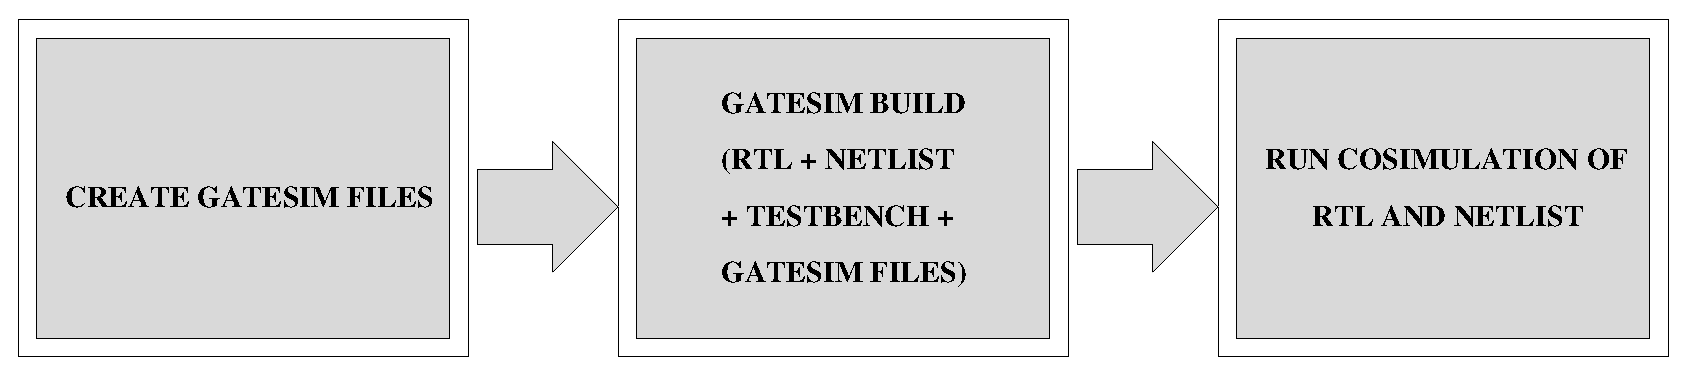
\includegraphics[scale=0.65]{./figures/cosim_flow.ps}
\caption{Co-sim Based Gatesim Flow}
\label{fig:cosim_flow.ps}
\end{figure}

Major steps involved in this flow are:

\begin{enumerate}
	\item \emph{\bf Getting gatesim files}

	Input to gatesims are obtained from LEC flow. The list includes the netlist file, files holding information regarding IO/Register mapping, gate defines, compare enables and testbench force files. These inputs from LEC stage are processed by a set of scripts for developing intermediate files which are needed by cosim build infrastructure. These files are exclusively required for netlist simulations and described below
	\begin{itemize}
		\item[{\bf gatesim.v}] instantiates top level netlist and ties its inputs with the behavioral RTL.
		\item[{\bf compare.v}] contains comparators those compare the outputs and register mappings, for each cycle of simulation.
		\item[{\bf forces.v}] contains all the force/release/assign commands for the gates corresponding to RTL force/release/assign statements. Forces are required in the design to shorten reset, initialize training parameters, initialize fuses among other things.
	\end{itemize}

	\item \emph{\bf Getting gatesim build} 

	Next stage is to enable a build structure supporting the co simulation of RTL and Netlist. The build includes:
	\begin{itemize}
		\item[-]Netlist to be verified
		\item[-]Complete RTL of SoC
		\item[-]Test bench components in its entirety
		\item[-]Gatesim files
	\end{itemize}

	\item \emph{\bf Run cosimulation of RTL and netlist}

	Running co-simulation is very similar to running RTL simulation. Output files include $<$testname$>$.out which contains the simulation transcript of the entire test and $<$testname$>$.fsdb (waveform dump file). The simulation transcript also contains gatesim errors called as ``miscompares''.
\end{enumerate}


As the netlist stimulus is obtained from a live RTL instead from stored vectors, cosim based gatesim overcame the biggest limitation associated with dual-sim. Over time, some good set of scripts aiding testbench generation, force generation were standardized. This method became the standard method for gatesims, close to a decade.

\subsection {LIMITATIONS OF CO-SIM METHODOLOGY}

Co-sim based Gatesim overcame all known limitations associated with early methodology. As design complexity grew, it brought in new set of unforeseen limitations. Of those, the important ones are already discussed in Section~\ref{intro:sec:ifg}.

In order to better understand these limitations certain experimental analysis were done. Experiments showed that the simulation performance of gatesim was affected sometimes as low as $10\%$ with respect to its counterpart RTL simulations. This indicates that:

\begin{itemize}
	\item[-]RTL Simulations contribute major to simulation performance than netlist.
	\item[-]Simulator spends more time in simulating RTL and verification components than netlist.
\end{itemize}

On further investigation it became clear that RTL simulation, which is simulated redundantly for the sole purpose of generating test vectors influences the simulation performance greatly. Such complex SOC design has multitude of Verification components in different programming languages including C, C++, SVTB, OVA, SVA and that these verification components take a big share of simulation cycles and have negative effect on simulation performance.

Evidently it was not an appropriate use of compute resources by having live RTL simulation every time, for the sole purpose of test vector generation. The analysis provides convincing evidence for us to attempt changes in existing cosim-based methodology.

 

%%%%%%%%%%%%%%%%%%%%%%%%%%%%%%%%%%%%%% IMPROVED DUAL-SIM APPROACH TO GATESIM %%%%%%%%%%%%%%%%%%%%%%%%%%%%%%%%
\newpage
\chapter{IMPROVED DUAL-SIM APPROACH TO GATESIM}
\label{chap:dualsim.tex}
After analyzing limitations associated with \emph{early dual-sim approach} it could be inferred that the main cause of inefficiency was the method used to capture, store, and apply test-vectors onto the netlist. Analyzing limitations associated with \emph{co-sim approach}, it could be inferred that the cause was bulky test-bench components associated with RTL simulations. Hence an improved solution would contain minimal testbench components retained and have an efficient method to capture, store, and apply test-vectors. 

Test-vectors are nothing but signal values at specific point in time. There are already different formats to store this information efficiently. FSDB \nomenclature{FSDB}{Fast Signal Database} is one such format. Hence it was suggested to improve gatesim methodology using FSDB itself as the format to store test-vectors. The proposed solution should also improve on

\begin{description}
	\item[Storage requirements]: Ensuring that storage resources are effectively used
	\item[Turn-around times]: Should avoid re-build for different test-vectors
\end{description}

FSDB\cite{SS:Verdi} or Fast Signal Database is a signal data file, similar to VCD\cite{ieee:v:2005} \nomenclature{VCD}{Value Change Dump} but much more compact. This format is in wide use across industry. Quick analysis revealed that FSDB as input test-vectors could be accomplished. Existing API's \nomenclature{API}{Application Programming Interface} provided by Verdi\cite{SS:Verdi} tool set for FSDB format could be used to retrieve values from FSDB. PLI$/$VPI\cite{ieee:v:2005} could be used to drive stimulus onto netlist.


The improved methodology becomes a dual-simulation methodology with two separate simulations.
\begin{enumerate}
	\item First simulation with non-gatesim components to generate the test-vectors in FSDB format.
	\item Second simulation with only gatesim components with capability to apply test-vectors from FSDB directly.
\end{enumerate}



\section {IMPROVED METHODOLOGY}
\label{sec:dualsim:im}
In dual simulation methodology the idea is to have two seperate simulations unlike co-sim. Both these simulations are completely independet except for the stimulus vector file. In the first unmodified RTL simulation (together with test bench components) dump is enabled in FSDB format. This FSDB dump is used as test-vectors for the following netlist simulation. In co-simulation methodology the same test bench will provide stimulus to RTL and netlist. ~\figurename{~\ref{fig:gatesim_flow.ps}} shows a flow diagram of proposed dual-sim methodology.  
\begin{figure}[h]
\centering
\includegraphics[scale=0.55]{./figures/gatesim_flow.ps}
\caption{Dual Sim}
\label{fig:gatesim_flow.ps}
\end{figure}

Stages associated with this methodology are
\begin{description}
	\item[RTL simulation] RTL simulation along with test bench components is already being done as part of functional verification. For gatesims, no changes are required except that the simulation signals needs to be dumped into FSDB, through runtime switches. Such FSDB stimulus vectors have to be generated for every stimulus envisioned to be applied onto the netlist. Note that once generated, the stimulus could be reused for repetitive netlist simulations.
	\item[Gatesim infrastructure] As in the case of co-simulation, gatesim files need to be generated from files obtained from LEC flow. Same infrastructure used in co-sim is used for this and hence no additional effort is required when the methodology is modified. Note that this step needed to be done only once.
	\item[Gatesim Build] Gatesim build could be obtained after compiling and elaborating the design netlist and infrastructure files with a simulator. The build would be devoid of RTL design and non-gatesim verification infrastructure. Note that this step needed to be done only once.
	\item[Gatesim simulation] Run all envisioned stimulus vectors onto the netlist.
\end{description}


{\bf VCS}: VCS is a high-performance Verilog simulator that  incorporates advanced, high-level abstraction verification  technologies into a single open native platform. VCS provides a fully featured implementation of Verilog language as defined in the {\it IEEE Standard Hardware Description Language} based on {\it Verilog Hardware Description Language (IEEE Std 1364-1995)} and {\it Standard Verilog Hardware Description Language (IEEE Std 1364-2001)}. It supports almost all verification, design and assertion constructs of {\it System Verilog}. It also provides native interfaces like DKI\nomenclature{DKI}{Direct C Kernel Interface} etc. VCS is a compiled code simulator and is widely considered as one of the advanced simulators avialable in the industry.

For this project we had used {\it VCS Verilog simulator} developed by {\it Synopsys Inc.} for RTL as well as netlist simulations. \figurename{\ref{fig:RTL_sim.eps}} is a self explainatory depction of RTL simulation. The implementation details of this methodology is detailed in following sections. 

\begin{figure}[h]
\centering
\includegraphics[scale=0.5]{./figures/RTL_sim.ps}
\caption{RTL Simulation}
\label{fig:RTL_sim.eps}
\end{figure}


\subsection{NETLIST SIMULATION FLOW}
\figurename{\ref{fig:netlist_sim.ps}} shows netlist simulation flow. Process~\textcircled{a} is generation of FSDB stimulus, which is already explained in Section~\ref{sec:dualsim:im}. Process~\textcircled{b} is intricated and is detailed in Section~\ref{sec:dualsim:sa}. Remaining process stages are explained here.

\begin{figure}[h]
\centering
\includegraphics[scale=0.65]{./figures/netlist_sim.ps}
\caption{Netlist Simulation}
\label{fig:netlist_sim.ps}
\end{figure}

Process stages of netlist simulation flow are:
\begin{enumerate}
	\item Obtain test-vectors in FSDB format
	\item Drive stimulus onto a dummy-RTL
	\item Dummy-RTL drives stimulus onto netlist
	\item Apply appropriate force signals from FSDB on to the dummy-RTL, which then forces it onto appropriate netlist nodes.
	\item Accomplish verification goals by clock-cycle-based-comparators connected between golden RTL reference and corresponding netlist nodes.
\end{enumerate}

\subsection{DUMMY-RTL}
When test-vectors were applied from FSDB to {\it Verilog} design, it was found that VPI/DKI method of stimulus application is not suitable when driving {\it Verilog} nets. Nets have special behaviour that they needs to be continuously dirven, which in the case of VPI/DKI is through forcing the net. But it was found to have flaky behaviour. Hence it was decided to create a ``dummy-RTL'' module that would contain all the signals those need to be export out of FSDB. These signals would have same size as their actual counterparts but be of type {\it Verilog} ``reg''. Test-vectors from FSDB would be applied to these signals inside dummy-RTL. \figurename{\ref{fig:dummy.ps}} shows a code snippet of dummy-RTL module (Process~\textcircled{c} in \figurename{\ref{fig:netlist_sim.ps}}). All wires, IO signals are of type ``reg'' in dummy-RTL module.


\begin{figure}[h]
\centering
\includegraphics[scale=0.75]{./figures/dummy.ps}
\caption{Dummy-RTL}
\label{fig:dummy.ps}
\end{figure}

\subsection{SIMULUS APPLICATOR}
Stimulus from dummy-RTL module is applied onto netlist by {\it Verilog} by connecting ports of netlist while instantiation at gatesim test-bench. ~\figurename{~\ref{fig:instant.ps}} gives a snippet of this Verilog instantiation of netlist module. There could be certain forces required in certain logic inside netlist, which is accomplished through {\it Verilog}'s ``force'' statement. These forces could be for initialisation, fuses or for hastening reset release.

\begin{figure}[h]
\centering
\includegraphics[scale=0.75]{./figures/instant.ps}
\caption{Netlist Instantiation}
\label{fig:instant.ps}
\end{figure}

\subsection{NETLIST SIMULATION}
Process~\textcircled{e} is simulation with netlist testbench components. These components are reused form of co-simulation methodology's netlist components (Section~\ref{sec:method:csgs}), with references of actual RTL paths changed to {\it Dummy-RTL}'s paths. Waveform dump needs to be enabled during simulation to enable debug in case of failure. Reference RTL waveform dump file is already available for the user.

\subsection{FUNCTION COMPARATORS}
Process~\textcircled{f} are a set of comparators those keep checking the behaviour of netlist with respect to RTL on every clock-cycle. Generally the comparision is made on respective active clocks, well after all signal changes have died down. The reference RTL signal is available in the dummy-RTL. Comparators may also consider certain important internal nodes, hence those have to be available in dummy-RTL as well. ~\figurename{~\ref{fig:compare.ps}} is a demo code representing a single comparator. Whenever compare fails, a ``miscompare'' information is written on to simulation transcript, that would aid debug. When test completes without any ``miscompare'' report, then test is said to have completed without failures.

\begin{figure}[h]
\centering
\includegraphics[scale=0.75]{./figures/compare.ps}
\caption{Cycle Compare Output Signals}
\label{fig:compare.ps}
\end{figure}


\section{STIMULUS APPLICATOR}
\label{sec:dualsim:sa}
Process~\textcircled{b} is a layered software infrastructure for the purpose of stimulus application onto the dummy-RTL. ~\figurename{~\ref{fig:fsdb.ps}} shows four different layers of the applicator. Together they accomplish transporting vector stimulus from FSDB file and finally delivering it to the netlist simulation. The first layer used to access FSDB file is provided by {\it Verdi} tool itself. It is available as a pre-built object\cite{Verdi:FsdbReader}, which could be linked with. The remaining three-layers of the infrastructure has been developed as part of this project and implemented as {\it C} and {\it C++} code.

\begin{figure}[h]
\centering
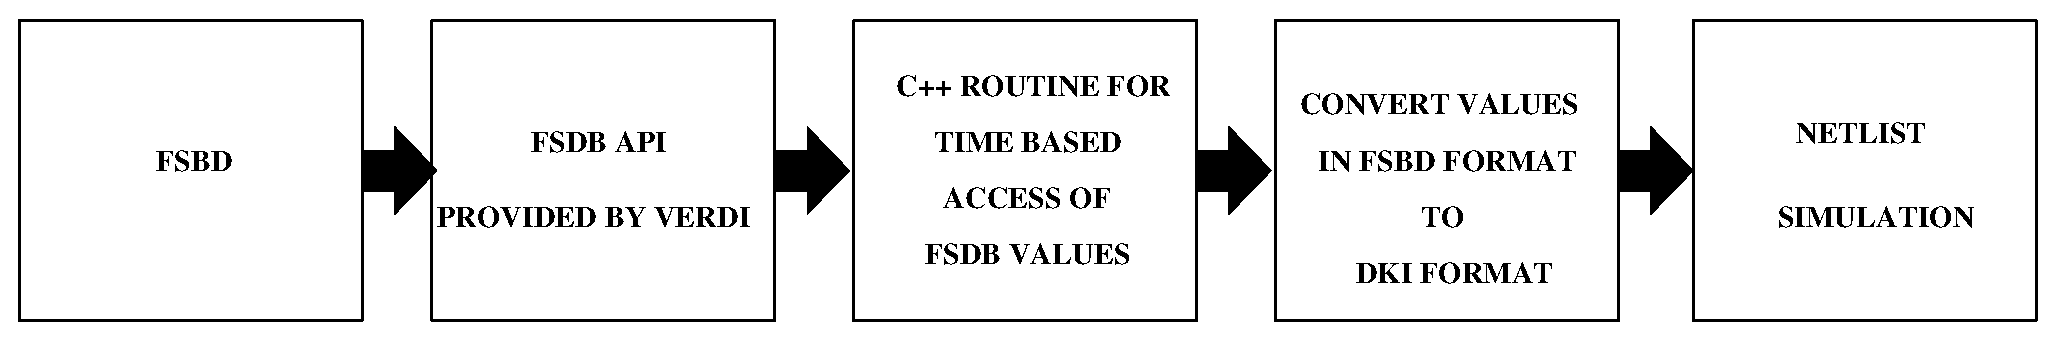
\includegraphics[scale=0.65]{./figures/fsdb.ps}
\caption{Accessing FSDB Signals}
\label{fig:fsdb.ps}
\end{figure}

\subsection{EXTRACTING STIMULUS}
FSDB is a binary file format for storing signal value change information. This format commonly used across the {\it Verdi} toolset and no other program has enough information to decode data from those files. But {\it Verdi} toolset, provides APIs\cite{Verdi:FsdbReader} \nomenclature{API}{Application Programmer's Interface} to be interfaced with. This project make use of those APIs, to accomplish desired task of accessing design signals at any point in time.

\begin{figure}[h]
\centering
\includegraphics[scale=0.65]{./figures/verdi.ps}
\caption{API For Accessing FSDB Signals}
\label{fig:verdi.eps}
\end{figure}

In order to successfully extract signal values from stored FSDB file the following needs to be done
\begin{enumerate}
\item[Handle FSDB file] In this process approprite FSDB file needs to be ``opened'' and be ``closed'' after all operations are completed. {\it Verdi} provides routines \textt{ffrOpen()/ ffrOpen2()} and \textt{ffrClose()} for these purposes respectively.
\item[Obtain signal handle] In this process handle to signals of interest needs to be obtained through APIs. Sample routine \textt{MyTreeCBFunc}\cite[p.~3]{Verdi:FsdbReader} is already provided by {\it Verdi}.
\item[Access signal values] Once signal handle is obtained, the signal's value at this point in time could be obtained by routine \textt{ffrGetVC()}.
\end{enumerate}

\subsection{TIME BASED TRAVERSAL}
\begin{figure}[h]
\centering
\includegraphics[scale=1]{./figures/time_access.ps}
\caption{Time Based Application of Stimulus}
\label{fig:dualsim:tbas}
\end{figure}

\figurename{\ref{fig:dualsim:tbas}} shows sequences of actions that would occur during simulation. At any simulation time `M', it would be required to apply the stimulus to all signals of interest. After  this, control is transferred to simulator which computes  the states values at time `M'. The event driven simulation  would proceed in this fashion for all subsequent event times until it reaches the next stimulus point `N'. Series of actions that took place for time `M' would be repeated for time `N'  and so forth.

List of RTL signals those need to be extracted would be refined over time, as netlist becomes stable. In this particular application, it would  be required  to obtain values of all signals of interest at the desired  instant. This type of traversal is called as time-based-traversal. Sample routine \textt{tb.cpp}\cite[p.~28]{Verdi:FsdbReader} is already provided by {\it Verdi}. In this application, a larger C++ infrastructure is required to be built since
\begin{enumerate}
\item Number of RTL signals those needs to be extracted is huge. Hence a seperate data structure is required.
\item Accessing of signal values in time-based fashion could be abstracted out.
\item Signal sizes vary from 1 to hundredes, so handling of different sized signals could be made uniform by {\t C++} routine abstraction.
\end{enumerate}


\subsection{VALUE CONVERSION TO DKI}
FSDB exports signals values in its custom 8-bit format, but that can't be used directly by any simulator. These values needs to get converted to a format that could be understood by the simulator. {\it Verilog} language\cite{ieee:v:2005} provides many standard interfaces such as PLI, VPI (or PLI 2.0) for this purpose. The drawback with these standard interfaces are that they are too slow when huge vectors are in consideration (like gatesims). Conversions to and from string based format is very timeconsuming as it was observed.

In order to overcome these limitations, VCS provides a non-standard interface called as DKI \nomenclature{DKI}{Direct-C Kernel Interface}. This interface has the advantage of less simulation overhead and smaller memory footprint compared to VPI interface. Hence DKI was choosen for this project.

\begin{figure}[h]
\centering
\includegraphics[scale=1]{./figures/dki.ps}
\caption{FSDB Format to DKI format}
\label{fig:dki.eps}
\end{figure}

Signal values could be retrived through {\it Verdi} APIs, as listed in speudo-code below.
\begin{verbatim}
  byte_T *vc_ptr;
  /* vc_ptr should be assigned to particular signals value change */

  // convert verilog bits to unsigned int
  uint retVal=0;
  uint8 bit;
  for (int i=0; i<=(msb-lsb); i++) {
    bit = vc_ptr[i+LBit-msb];
    retVal = (retVal<<1)
           | (bit==FSDB_BT_VCD_1 || (bit==FSDB_BT_VCD_X));
  } 
\end{verbatim}
DKI provides direct interface to internal representation of any simulator object. Such retrieved signal values could be assigned to VCS's object as per instructions in {\it VCS User Guide}\cite[Section~C~Language~Interface>~Direct~C]{VCS:vcs.pdf}.

\subsection{INTERACTION WITH SIMULATOR}

The C++ infrastructure will open the FSDB file and initiate a playback through the file. Whenever a signal that is attached using APIs changes, the C++ will identify this and will ensure the changed value is made available to the netlist simulation.  Figure x shows the complete flow of the C++ routine developed for FSDB signal access, conversion and application onto Verilog component.


\begin{figure}[h]
\centering
\includegraphics[scale=1]{./figures/cpp.ps}
\caption{C++ Routine for FSDB Signal Extraction}
\label{fig:cpp.eps}
\end{figure}

A set of RTL signal accessed at time based manner and applied onto netlist is effectively doing the job of test-vectors as vectors are nothing but signal values at different instants of time.
Once signals are accessed from FSDB file by API's and C++ routine developed next step is applying it onto netlist. However Verilog based netlist cannot directly interact with extracted FSDB format objects. For this a conversion stage is required.  

Whenever the C++ moves in time and identify a change in signal value in FSDB signal, an assign statement will assign the new FSDB signal value to DKI signal object.  These DKI signals can drive Verilog signals by using "{\emph Attach}" routine provided by API, that ties together DKI object with RTL signal. 

In the previous section we have discussed extracting FSDB, accessing it in a time based manner and converting it to a format that can interact with Verilog. Next step is using these signals for netlist simulation.

 


%%%%%%%%%%%%%%%%%%%%%%%%%%%%%%%%%%%%%% RESULTS %%%%%%%%%%%%%%%%%%%%%%%%%%%%%%%%%%%%%%%%%%%%%%%
\newpage
\chapter{RESULTS}
\label{chap:results.tex}
A new gate simulation flow based on separate simulation of RTL and netlist was developed. Performance analysis was done with respect to co-sim methodology. A set of standard test cases were considered for the purpose. An exclusive machine was used for benchmarking and hence tests were run in sequence one after the other in both the methodologies. The machine features were:
\begin{itemize}
\item Linux 2.6.18-308.1.1.el5
\item Authentic AMD family F model 1 stepping 2
\item AMD FX(tm)-8150 Eight-Core Processor
\item MemTotal:     32925800 kB
\end{itemize}  

~\tablename{~\ref{tab:Simulation Performance}} compares simulation performances whereous ~\tablename{~\ref{tab:Memory Requirement}} compares simulation memory requirement.
%%%%%%%%%%%%%%%%%%%%%%%%%%%%%%%%%%%%%%%%%%%%%%%%%%%%%%%%%%%%%%%%%%%%%%%%%%%%%%%%%


%%%%%%%%%%%%%%%%%%%%%%%%%%%%%%%%%%%%%%%%%%%%%%%%%%%%%%%%%%%%%%%%%%%%%%%%%%%%%%%%%
\newpage
\section{SIMULATION PERFORMANCE ANALYSIS}
\begin{table}[h!]
\begin{center}
\caption{Simulation Performance Comparison}
\label{tab:Simulation Performance}
\vspace{0.2cm}
\begin{tabular}{|l|r|r|r|}
\hline
\multirow{3}{*}{\bf Stimulus} & &	&\\ & {\bf Co-sim Simulation} 	& {\bf Dual-sim Simulation} & {\bf Improvement } 	\\ & {\bf Time (in sec)}  &  {\bf Time (in sec)} &  {\bf(X times) }\\



%\multirow{2}{*}{\bf Stimulus}	&\multirow{2}{*}{\bf Co-sim Simulation Time (in sec)}	&\multirow{2}{*}{\bf Dual-sim Simulation Time (in sec)}	&\multirow{2}{*}{\bf Improvement (X times)} 		\\
						&				&				&				\\
\hline
Pattern 1 			&821245				&79965				&10.27 				\\
Pattern 2  				&883227				&85731				&10.3 				\\

Pattern 3  		&854760				&83083				&10.28				\\

Pattern 4  			&456881				&46071 				&9.91				\\

Pattern 5  				&709871				&69605				&10.19				\\
\hline


\end{tabular}
\end{center}

\end{table}



\section{MEMORY REQUIREMENT}
\begin{table}[h!]
\begin{center}
\caption{Simulation Memory Requirement}
\label{tab:Memory Requirement}
\vspace{0.2cm}
\begin{tabular}{|l|r|r|r|}
\hline
\multirow{3}{*}{\bf Stimulus} & &	&\\ & {\bf Co-sim Simulation} 	& {\bf Dual-sim Simulation} & {\bf Improvement } 	\\ & \bf{Mem Req (in Mb)}  &  {\bf{Mem Req (in Mb)}} &  {\bf(X times) }\\



%\multirow{2}{*}{\bf Stimulus}	&\multirow{2}{*}{\bf Co-sim Simulation Time (in sec)}	&\multirow{2}{*}{\bf Dual-sim Simulation Time (in sec)}	&\multirow{2}{*}{\bf Improvement (X times)} 		\\
						&				&				&				\\
\hline
Pattern 1 			&1103.9				&98.8				&11.17 				\\

Pattern 2  				&1103.9				&98.8				&11.17				\\

Pattern 3  		&1105.1				&98.8				&11.18				\\

Pattern 4  			&1103.3			&98.8 				&11.17				\\

Pattern 5  				&1103.3				&98.8				&11.17				\\
\hline


\end{tabular}
\end{center}

\end{table}
 

%%%%%%%%%%%%%%%%%%%%%%%%%%%%%%%%%%%%%% CONCLUSION %%%%%%%%%%%%%%%%%%%%%%%%%%%%%%%%%%%%%%%%%%%%%%%
\newpage
\chapter{CONCLUSION}
\label{chap:conclusion}
A new dual-sim or sim after sim flow for gatesim was developed. Simulation performance when benchmaked and compared against current co-simulation method on a dedicated machine, shows a consistent improvement of around 10. Use of FSDB as the source of test vectors helps to keep the disk requrirement minimal and to get rid of bulky time hogging test bench components. The methodology also enables quicker turn-around time. This 10 times improvement in simulation performance will help in aiding time-to-market of cutting-edge processors. The method still requires a one time RTL simulation runs for generating stimulus (as FSDB). The proposed methodology needs minor modifications to existing co-simulation methodology and hence could be adopted to new projects with ease.

Though the improved methodology is dependent on vectors from RTL simulations and is not independent by itself, gains obtained in turn-around times were considerable, and is a good return-on-investment when complete gatesim verification is considered.

\paragraph{Potential for future work:}Observed performance of improved dual-sim methodology could be further increased by optimizing glue code used for reading FSDB and applying that inside design. Infrastructure created during the course of this project could be packaged into libraries to simplify porting between projects.



%\chapter{REFERENCES}
\bibliographystyle{nitk}
%\begin{thebibliography}{10}
%\providecommand{\url}[1]{#1}
%\csname url@rmstyle\endcsname
%\providecommand{\newblock}{\relax}
%\providecommand{\bibinfo}[2]{#2}
%\providecommand\BIBentrySTDinterwordspacing{\spaceskip=0pt\relax}
%\providecommand\BIBentryALTinterwordstretchfactor{4}
%\providecommand\BIBentryALTinterwordspacing{\spaceskip=\fontdimen2\font plus
%\BIBentryALTinterwordstretchfactor\fontdimen3\font minus
%  \fontdimen4\font\relax}
%\providecommand\BIBforeignlanguage[2]{{%
%\expandafter\ifx\csname l@#1\endcsname\relax
%\typeout{** WARNING: IEEEtran.bst: No hyphenation pattern has been}%
%\typeout{** loaded for the language `#1'. Using the pattern for}%
%\typeout{** the default language instead.}%
%\else
%\language=\csname l@#1\endcsname
%\fi
%#2}}

\bibitem{ieee:SOC:2010}
Brackenbury, Linda EM, Luis, A. Plana \& Jeffrey Pepper. (2010). System-on-Chip design and implementation. {\it Education, IEEE Transactions}. v~53, no.~2, pp. 272-281.

\bibitem{soc}
Mosensoson, Guy,``Practical approaches to SoC verification.''\emph{In Proceedings of DATE User Forum,} pp. 05-08. 2002.

\bibitem{phd:zhang}
Zhang, L. (2005),`` Design Verification for Sequential Systems at Various Abstraction Levels,''\emph{Doctoral dissertation, Virginia Polytechnic Institute and State University,}2005.

\bibitem{ieee:segev:2004}
Segev, Eyal, Sharon Goldshlager, Hillel Miller, Oren Shua, Olga Sher, and Shlomo Greenberg,``Evaluating and comparing simulation verification vs. formal verification approach on block level design,'' \emph{In Electronics, Circuits and Systems, 2004. ICECS 2004. Proceedings of the 2004 11th IEEE International Conference},pp. 515-518, 2004.

\bibitem{ieee:formal:2004}
Tasiran, Serdar, Yuan Yu, and Brannon Batson,``Linking simulation with formal verification at a higher level,''\emph{Design and Test of Computers,} IEEE 21, no. 6, pp. 472-482,2004.

\bibitem{SS:AMD64-V1}
\BIBentryALTinterwordspacing
AMD Corporation (May 2011). ``Volume 1: Application Programming''. \emph{AMD64 Architecture Programmer's Manual}. AMD Corporation. Retrieved 2011-10-29.
\url{http://support.amd.com/us/Processor_TechDocs/24592_APM_v1.pdf}
\BIBentrySTDinterwordspacing
 
\bibitem{SS:AMD64-V2}
\BIBentryALTinterwordspacing
AMD Corporation (May 2011). ``Volume 2: System Programming''. \emph{AMD64 Architecture Programmer's Manual}. AMD Corporation. Retrieved 2011-10-29.
\url{http://support.amd.com/us/Embedded_TechDocs/24593.pdf}
\BIBentrySTDinterwordspacing
 
\bibitem{http:dygraphs}
\BIBentryALTinterwordspacing
Dygraphs. (2013, Jun.) {JavaScript Visualization Ligrary}. [Online]. Available:
  \url{http://dygraphs.com/}
\BIBentrySTDinterwordspacing


\bibitem{ieee:power:2009}
Zhang,~Y. and Zhang,~G. ``Fast gate-level simulation and power analysis for high performance microprocessor,'' in {\emph IEEE Computer Science and Education, 2009. ICCSE'09. 4th International Conference}, pp. 1155-1158, 2009.


\bibitem{ieee:v:2005}
  IEEE,
  \emph{``1364-2005 - IEEE Standard for Verilog Hardware Description
  Language''}.
	IEEE STANDARD,
	2005

\bibitem{ieee:sv:2009}
  IEEE,
	\emph{``1800-2012 - IEEE Standard for SystemVerilog--Unified Hardware Design,
  Specification, and Verification Language''}.
	IEEE STANDARD,
	2009

\bibitem{ieee:boolean}
Randal E. Bryant,
  ``Graph-Based Algorithms for Boolean Function Manipulation,'' \emph{IEEE Transactions on Computers}, vol.C ~35, no.~12, 1986.

\bibitem{lec}
McDonald, William, and Janny Liao,
	``Logic Equivalence Checking Has Arrived For FPGA Developers.`` \emph{Design and Verification Conference (DVCon)}, 2006.

\bibitem{SS:Verdi}
\BIBentryALTinterwordspacing
SpringSoft. (2013, May.) {Verdi Automated Debug System}. [Online]. Available:
  \url{http://www.springsoft.com/products/debug-automation/verdi}
\BIBentrySTDinterwordspacing

	
%\bibitem{compton2002reconfigurable}
%K.~Compton and S.~Hauck, ``Reconfigurable computing: a survey of systems and
%  software,'' \emph{ACM Computing Surveys (csuR)}, vol.~34, no.~2, pp.
%  171--210, 2002.
%
%\bibitem{P1171121623}
%M.~Ramesh~Kini and S.~Sumam~David, ``Asic implementation of address generation
%  unit for digital signal processing kernel-processor,'' \emph{ICGST
%  International Journal on Programmable Devices, Circuits and Systems, PDCS},
%  vol.~11, pp. 1--9, December 2011.
%
%\bibitem{graham1999reconfigurable}
%P.~Graham and B.~Nelson, ``Reconfigurable processors for high-performance,
%  embedded digital signal processing,'' in \emph{Proceedings of 9th
%  international workshop on Field Programmable Logic and Applications}.\hskip
%  1em plus 0.5em minus 0.4em\relax Springer, 1999, pp. 1--10.
%
%\bibitem{ramesh2009comprehensive}
%M.~Ramesh~Kini and S.~Sumam~David, ``Comprehensive address generator for
%  digital signal processing,'' in \emph{Proceedings of International Conference
%  on Industrial and Information Systems (ICIIS 2009),Srilanka}.\hskip 1em plus
%  0.5em minus 0.4em\relax IEEE, 2009, pp. 325--330.
%
%\bibitem{huang2002reconfigurable}
%Z.~Huang and S.~Malik, ``Exploiting operation level parallelism through
%  dynamically reconfigurable datapaths,'' in \emph{Proceedings of the 39th
%  annual Design Automation Conference}.\hskip 1em plus 0.5em minus 0.4em\relax
%  ACM, 2002, pp. 337--342.
%
%\bibitem{SS:AMD64}
%\BIBentryALTinterwordspacing
%AMD64 Architecture Programmer's Manual Volume 1: Application Programming (2005, Nov)
%\url{http://www.serc.iisc.ernet.in/facilities/ComputingFacilities/systems/tyrone/Application\%20Programming.pdf}
%\BIBentrySTDinterwordspacing
\bibitem{SS:Cadence}
\BIBentryALTinterwordspacing
Cadence. (2013, Jan.) {Functional Verification Survey-{\emph Why Gate-Level Simulation is Increasing}}.[Online]. Available:
\url {http://www.cadence.com/Community/blogs}
\BIBentrySTDinterwordspacing

\bibitem{SS:Cadence-2}
\BIBentryALTinterwordspacing
Cadence. (2012, Jan.) {Gate-Level Simulation Methodology-{\emph Improving Gate-Level Simulation Performance}}.[Online]. Available:
\url {http://www.cadence.com/rl/Resources/white_papers/Gate_Level_Simulation_WP.pdf}
\BIBentrySTDinterwordspacing


\bibitem{Verdi:FsdbReader}
\BIBentryALTinterwordspacing
Novas. (2011, Oct.) [Tool Installation Resources]. Available:
  \verb|$VERDI_HOME/share/FsdbReader/doc/FsdbReader.pdf|
\BIBentrySTDinterwordspacing

\bibitem{VCS:vcs.pdf}
\BIBentryALTinterwordspacing
Synopsys. (2013, Dec.) [Tool Installation Resources]. Available:
  \verb|$VCS_HOME/doc/UserGuide/pdf/vcs.pdf|
\BIBentrySTDinterwordspacing

\bibitem{wiki:2013:VPI}
\BIBentryALTinterwordspacing
Wikipedia. (2013, June.) {Verilog Procedural Interface}. [Online]. Available:
  \url{http://en.wikipedia.org/wiki/Verilog_Procedural_Interface}
\BIBentrySTDinterwordspacing

\bibitem{aw:2013:VPI}
\BIBentryALTinterwordspacing
Asic World. (2013, June.) {Verilog Procedural Interface}. [Online]. Available:
  \url{http://www.asic-world.com/verilog/pli6.html}
\BIBentrySTDinterwordspacing

\bibitem{aw:2013:vbooks}
\BIBentryALTinterwordspacing
Asic World. (2013, June.) {Verilog Books}. [Online]. Available:
  \url{http://www.asic-world.com/verilog/books.html}
\BIBentrySTDinterwordspacing

\bibitem{ss:pli:1999}
\BIBentryALTinterwordspacing
Sutherland, Stuart.  {\em The Verilog PLI Handbook: A User's Guide and Comprehensive
  Reference on the Verilog Programming Language Interface}.
\newblock Springer, 1999. Hardcover.
\newblock ISBN: 0-7923-8489-X.
\BIBentrySTDinterwordspacing

\bibitem{sm:pli:1999}
\BIBentryALTinterwordspacing
Mittra, Swapnajit.  {\em Principles of Verilog PLI}.
\newblock Springer, 1999. Hardcover.
\newblock ISBN: 0-7923-8477-6
\BIBentrySTDinterwordspacing

%\bibitem{tms320c55x2001programmer}
%T.~DSP, ``Programmer’s guide,'' \emph{SPRU376, Texas Instruments}, 2001.
%
%\bibitem{EDKconceptsUG683}
%Xilinx, ``Edk concepts, tools, and techniques,'' \emph{UG683 (v12.3), Xilinx},
%  Sept. 2010.
%
%\bibitem{chipscopeguideUG029}
%Xilinx, ``Chipscope pro 12.1 software and cores,'' \emph{UG029 (v12.1),
%  Xilinx}, Apr. 2010.
%
%\bibitem{dorairaj2005planahead}
%N.~Dorairaj, E.~Shiflet, and M.~Goosman, ``Planahead software as a platform for
%  partial reconfiguration,'' \emph{Xcell Journal}, vol.~55, pp. 68--71, 2005.
%
%\bibitem{oslibref}
%Xilinx, ``Xilinx OS and Libraries document collection,'' \emph{UG643, Xilinx},
%  April. 2012.

\end{thebibliography}

%\addcontentsline{toc}{section}{REFERENCES}
\bibliography{reference}{}

%%%%%%%%%%%%%%%%%%%%%%%%%%%%%%%%%%%%%% BIO DATA %%%%%%%%%%%%%%%%%%%%%%%%%%%%%%%%%%%%%%%%%%%%%%%%%%%%%
\newpage
\pagestyle{plain}

\section*{\centering BIODATA}
\begin{tabular}{lll}
%\begin{center}
Name			&:	&Meera Mohan			\\

Qualification 		&:	&B.Tech (Electronics and Communication)	\\

			&	&Mahatma Gandhi University, Kottayam			\\

Contact Address 	&:	&D/O Mohandas. E. K			\\
		
			&	&Margangattu House		\\
		
			&	&Memana, Oachira		\\

			&	&Kollam, Kerala-690526		\\

Contact Number  	&:	&7411352081				\\

Email id		&:	&miramohan@gmail.com			\\

%List of publications 	&:	&1					\\
%\end{center}
\end{tabular}
%\addcontentsline{toc}{section}{BIODATA}



%\hskip 1em plus
%  0.5em minus 0.4em\relax IEEE, 2009, pp. 325--330.

\end{document}          
